\label{ch:experimental_results}

\section{FTIR}
\label{sec:ftir_results}
Here are presented the FTIR spectra of a raw, ground and polished sample. 

\begin{figure}[H]
    \centering
    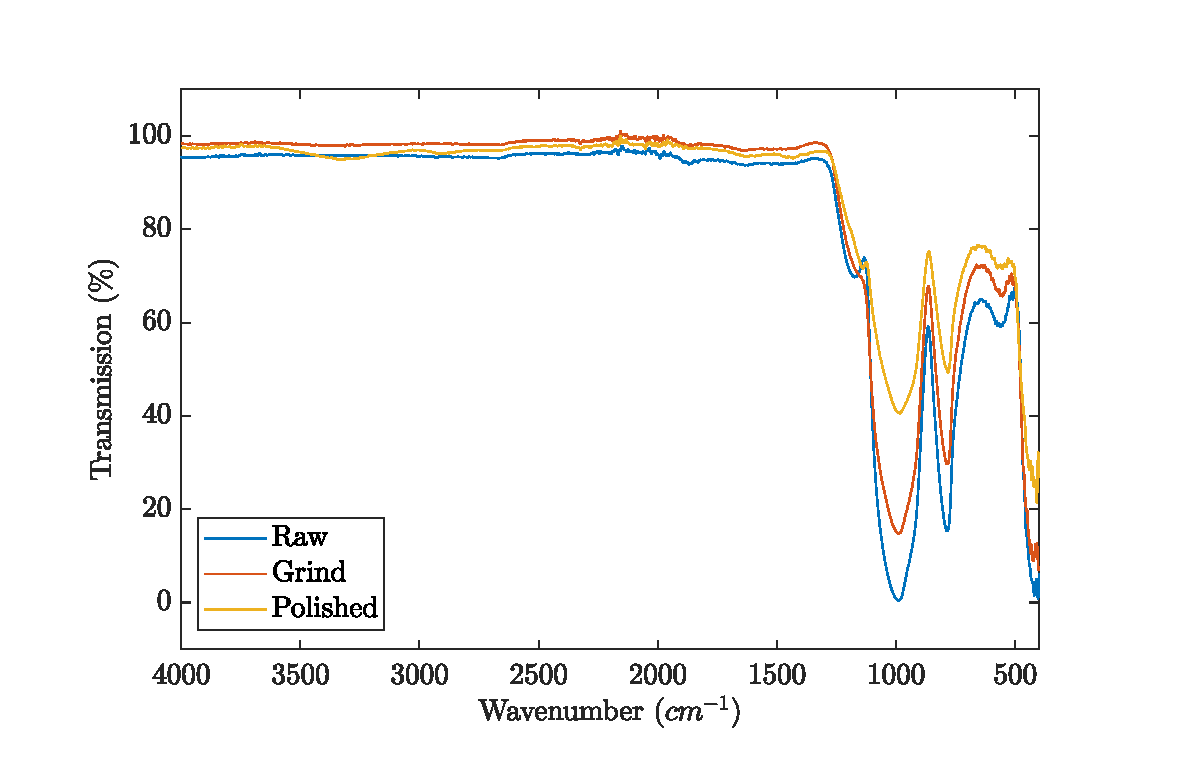
\includegraphics[width = \textwidth]{chapter_5/others/ftir_plot.pdf} 
    \vspace*{-30pt}
    \caption{FTIR spectra.}
    \label{fig:ftir_plot}
 \end{figure}
 As already said in Chapter~\ref{fig:ftir_issues} the differences in amplitude is not relevant for a measurement but only the position and presence of transmission dips. 
\\
From Figure~\ref{fig:table_inorganic} we can identify that the two major peaks present in the spectra, at $1000 \:cm^{-1} $and $780 \:cm^{-1}$, respectively corresponds to \ce{SiO2} and \ce{SiO3} compounds, obviously present in glass.
\\
\begin{figure}[H]
    \centering
    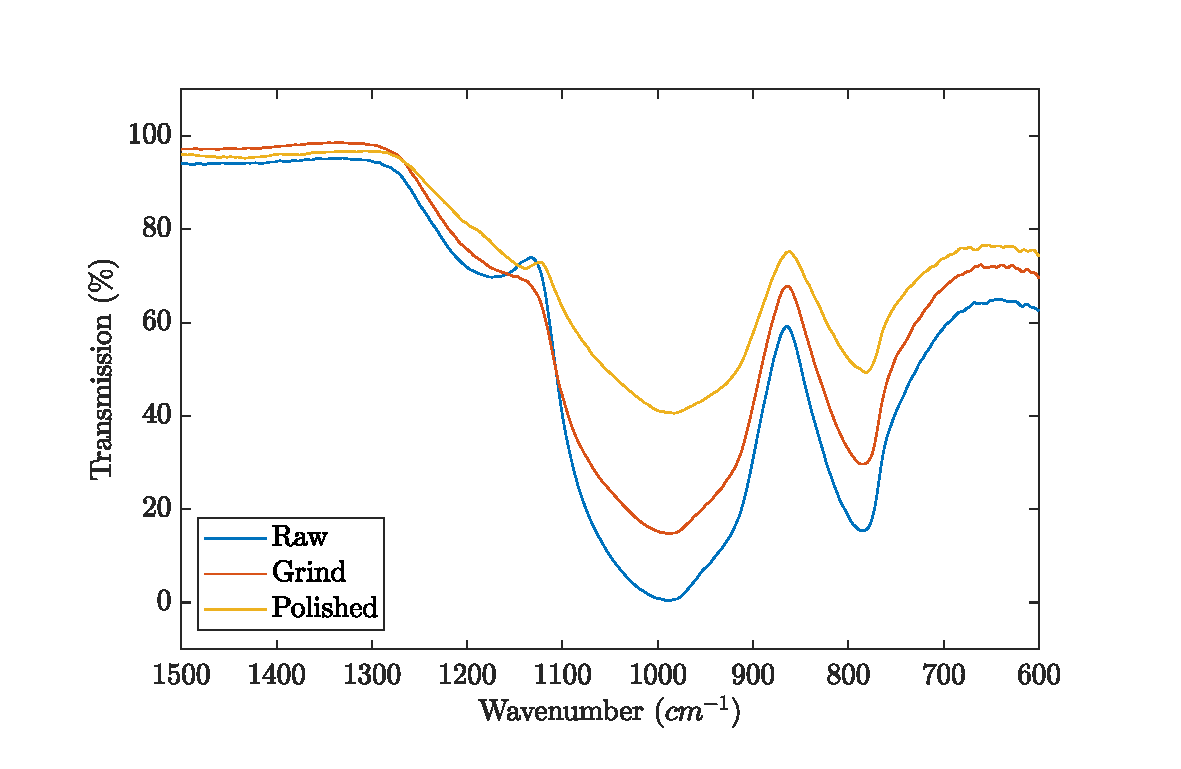
\includegraphics[width = \textwidth]{chapter_5/others/ftir_plot_zoom.pdf} 
    \vspace*{-30pt}
    \caption{Focus on the notable spectral range of the FTIR measurements.}
    \label{fig:ftir_zoom_plot}
 \end{figure}

The small dip at $1173 \:cm^{-1}$, that can be seen more clearly in Figure~\ref{fig:ftir_zoom_plot}, is associated to \ce{C-O} stretching and could be caused by carbonaceous compounds that are present on the surface as residues from the cutting process. The absorption, in fact, disappears for the ground and polished sample, showing that the contamination came from manufacturing, and was then removed with our procedures.
\\
This is in line from what has already been found here [paper robert kohler].

\section{Contact Angle Measurement}
Contact angle measurements were also performed on the raw and on a polished sample. The results are presented in the next figure.
\begin{figure}[H]
    \centering
    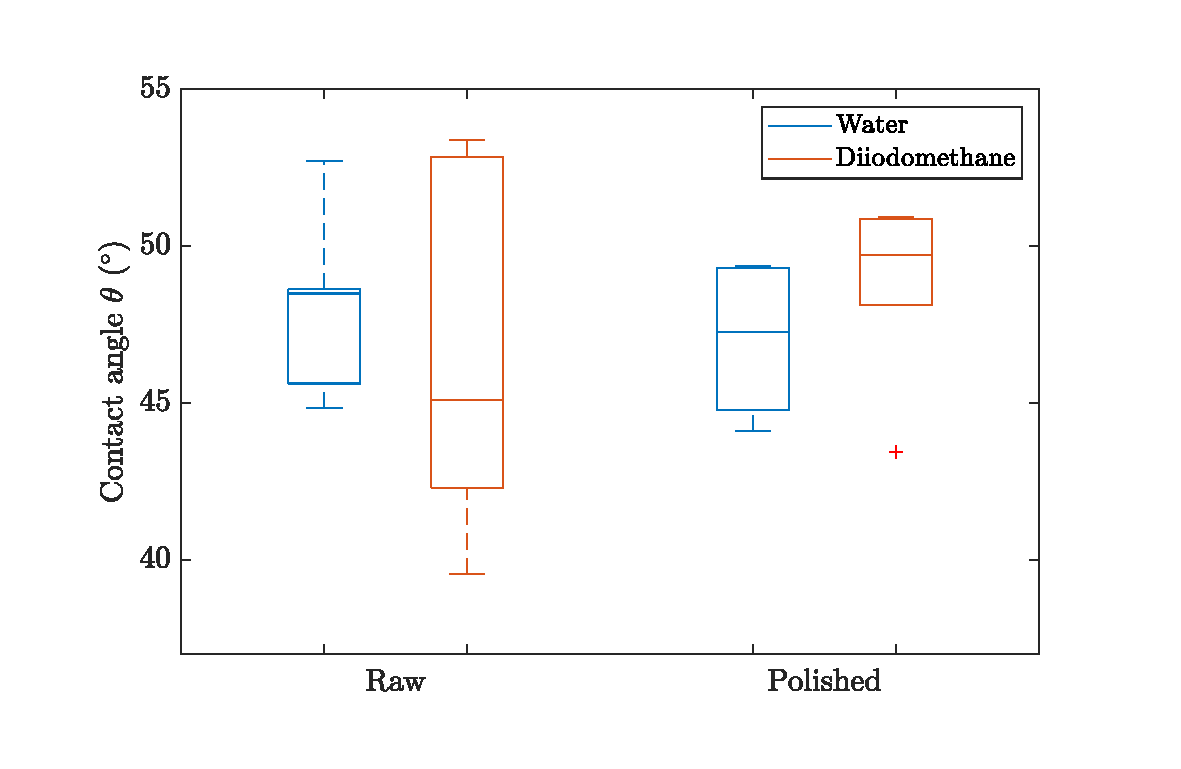
\includegraphics[width = \textwidth]{chapter_5/others/contact_angle.pdf} 
    \vspace*{-30pt}
    \caption{Contact angle measurements for a raw and a polished sample. }
    \label{fig:contact_angle_raw_polished}
 \end{figure}
Considering the differences in the average value of the measured angle between the polar and the non-polar probe liquids, there could be a change in the contributions to the surface energy of the glass. Specifically, it does not seem that the polar fraction of surface energy has been affected by the polishing. However, in the case of diiodomethane, both the mean and the standard deviation notably changed for the two sample. The shift in the mean can be explained by the presence of carbonaceous compounds on the surface of the glass as a side effect of the manufacturing process, supporting what has been found with FTIR measurements in Chapter~\ref{sec:ftir_results}.
\\
Contact angle values are also influenced by the roughness of the surface, this could explain the decrease in standard deviation of the polished sample.

\section{XPS}
\label{sec:xps_results}
XPS analyses was done to confirm the presence of the contaminants with a more precise technique, check for species that are not easily detectable by LIBS and to see if chemical shift is present in the spectra of aluminum and silicon. This would imply the formation of new chemical species during the polishing phase.
\\
The measurements were performed on raw and polished samples. The results are presented in the following figures.
\\


\begin{figure}[H]
   \centering
   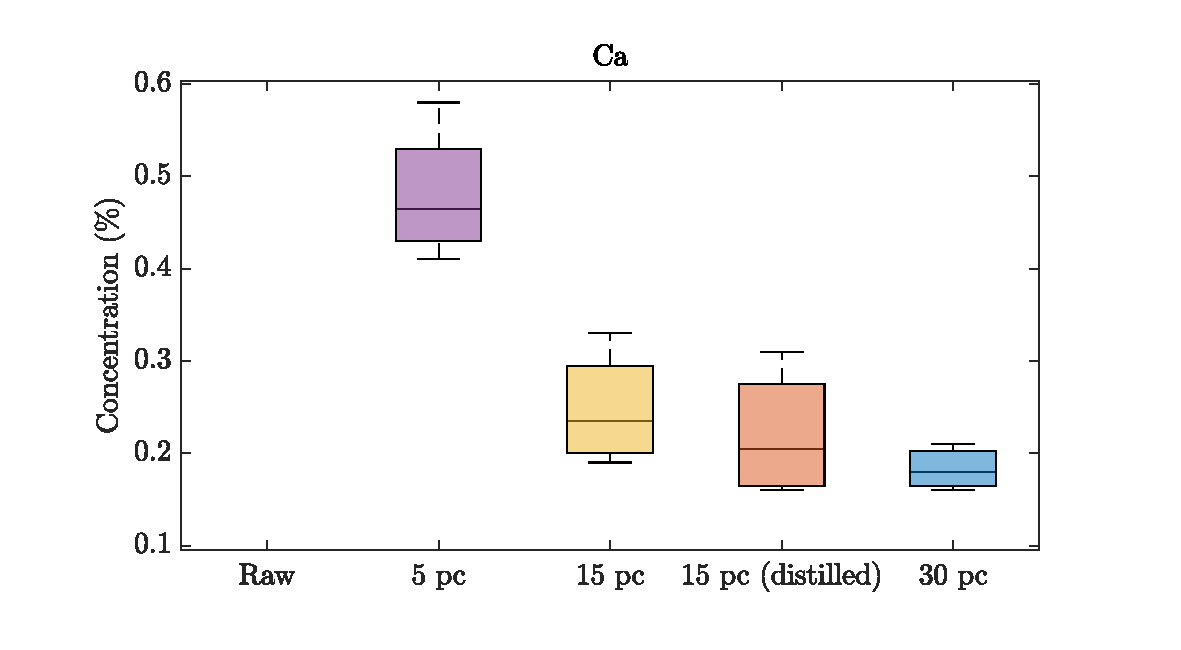
\includegraphics[width = \textwidth]{chapter_5/others/XPS/XPS_Ca_conc.pdf} 
   \vspace*{-30pt}
   \caption{Calcium concentration measured by XPS. }
   \label{fig:ca_xps}
\end{figure}


\begin{figure}[H]
   \centering
   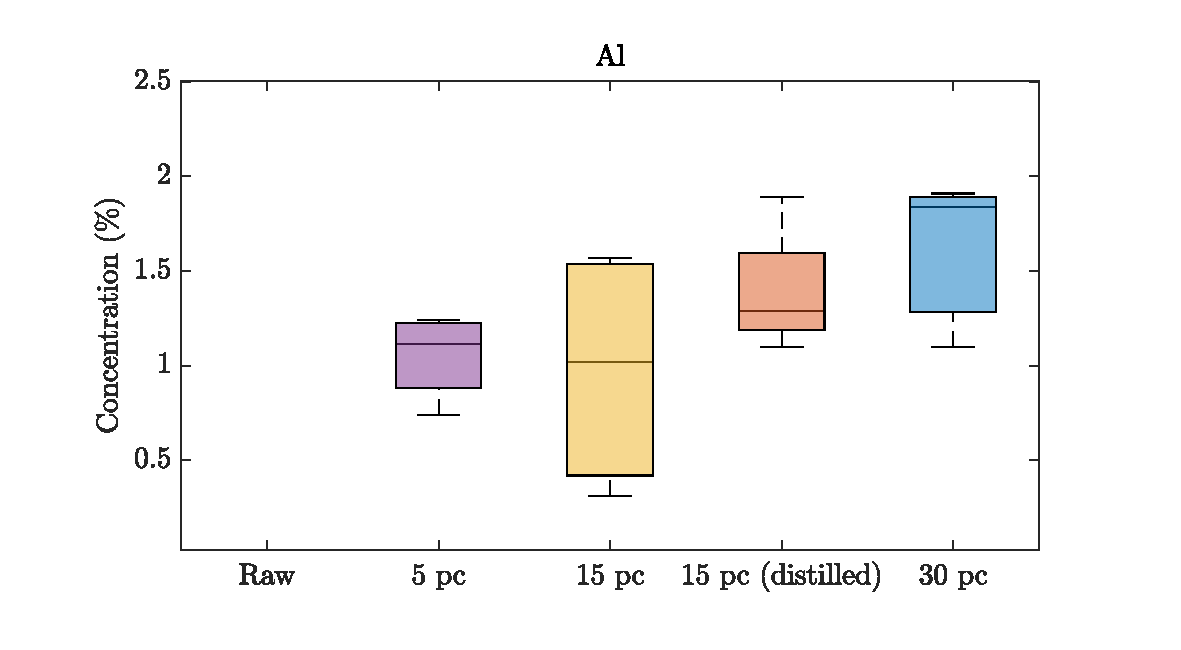
\includegraphics[width = \textwidth]{chapter_5/others/XPS/XPS_Al_conc.pdf} 
   \vspace*{-30pt}
   \caption{Aluminum concentration measured by XPS. }
   \label{fig:al_xps}
\end{figure}

\begin{figure}[H]
   \centering
   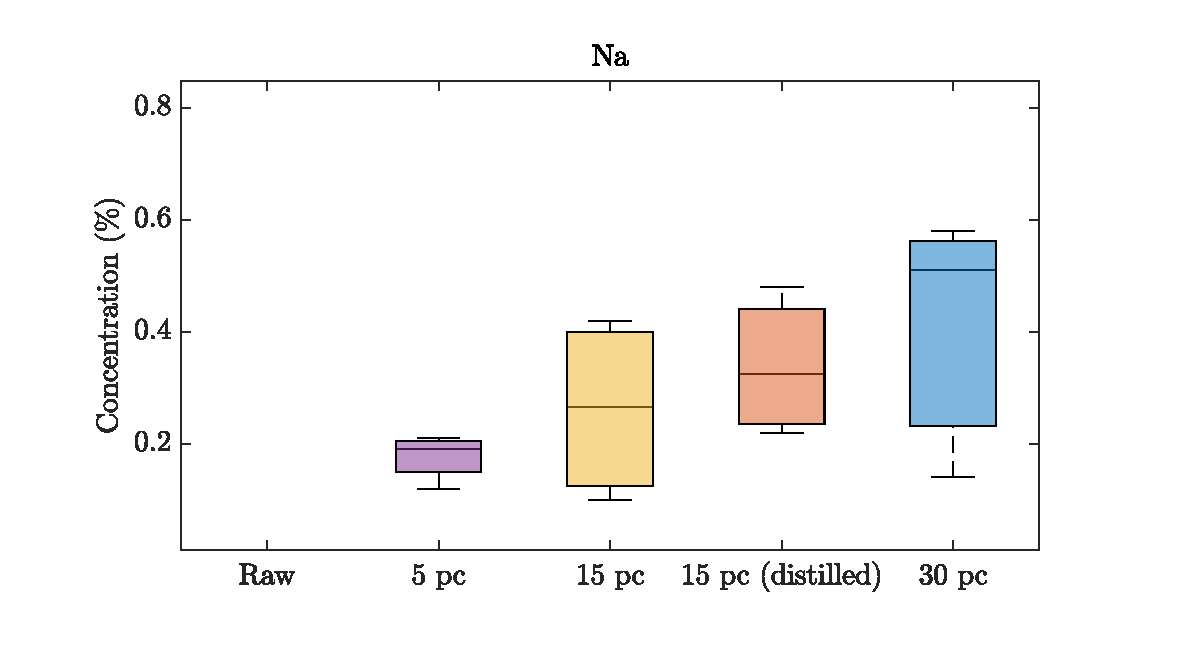
\includegraphics[width = \textwidth]{chapter_5/others/XPS/XPS_Na_conc.pdf} 
   \vspace*{-30pt}
   \caption{Sodium concentration measured by XPS. }
   \label{fig:na_xps}
\end{figure}


Calcium, aluminum and sodium impurities were found in the XPS measurements. In the case of aluminum and sodium, it appears that their concentration is increasing as the polish concentration increases. However, calcium present the opposite behavior.

\begin{figure}[H]
   \centering
   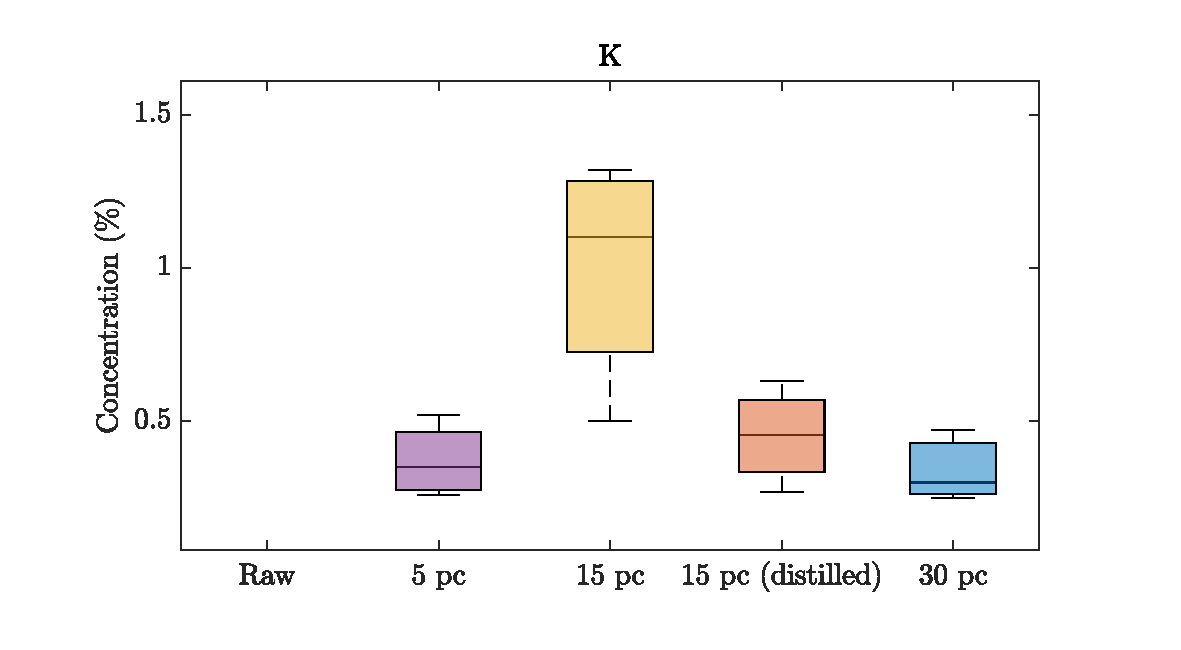
\includegraphics[width = \textwidth]{chapter_5/others/XPS/XPS_K_conc.pdf} 
   \vspace*{-30pt}
   \caption{Potassium concentration measured by XPS. }
   \label{fig:k_xps}
\end{figure}
\begin{figure}[H]
   \centering
   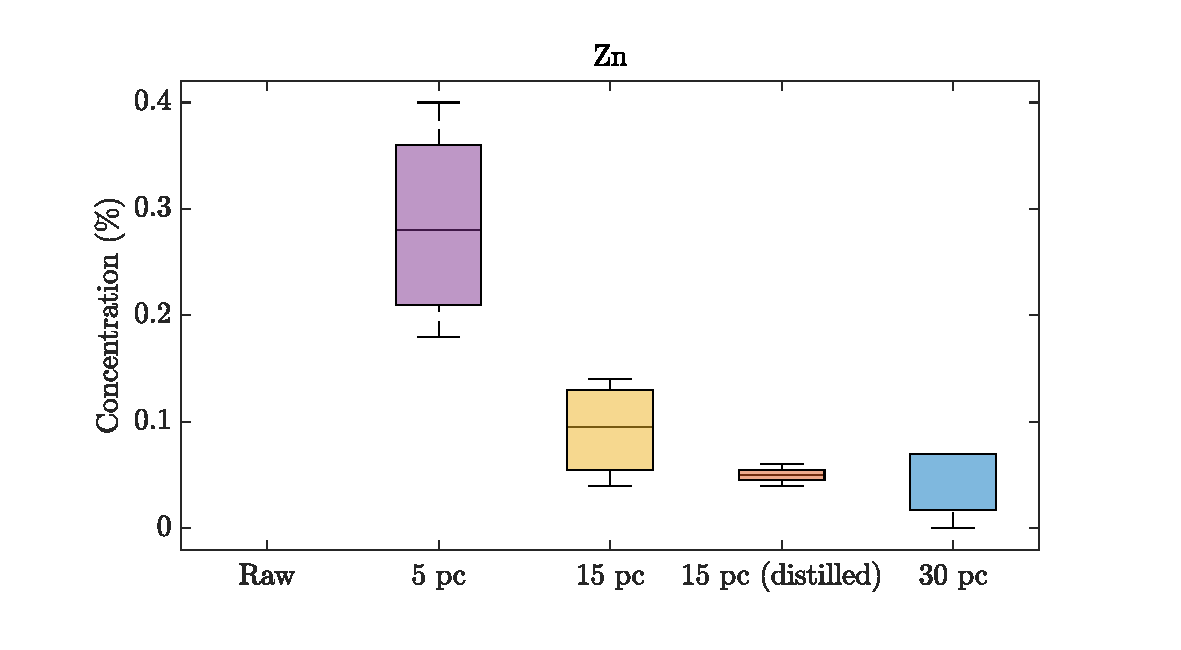
\includegraphics[width = \textwidth]{chapter_5/others/XPS/XPS_Zn_conc.pdf} 
   \vspace*{-30pt}
   \caption{Zinc concentration measured by XPS. }
   \label{fig:zn_xps}
\end{figure}

Traces of zinc and potassium have also been found, these species were never detected during our LIBS measurements. The potassium impurities were expected due to its presence in the tap water, as shown in Table~\ref{table:water_composition}.
\\
The dependence of Zinc relatively to the polish concentration has a decreasing behavior, similar to calcium.
\\
None of the contaminants were absent from the measurement of the samples polished with the solution made with distilled water.

\begin{figure}[H]
   \centering
   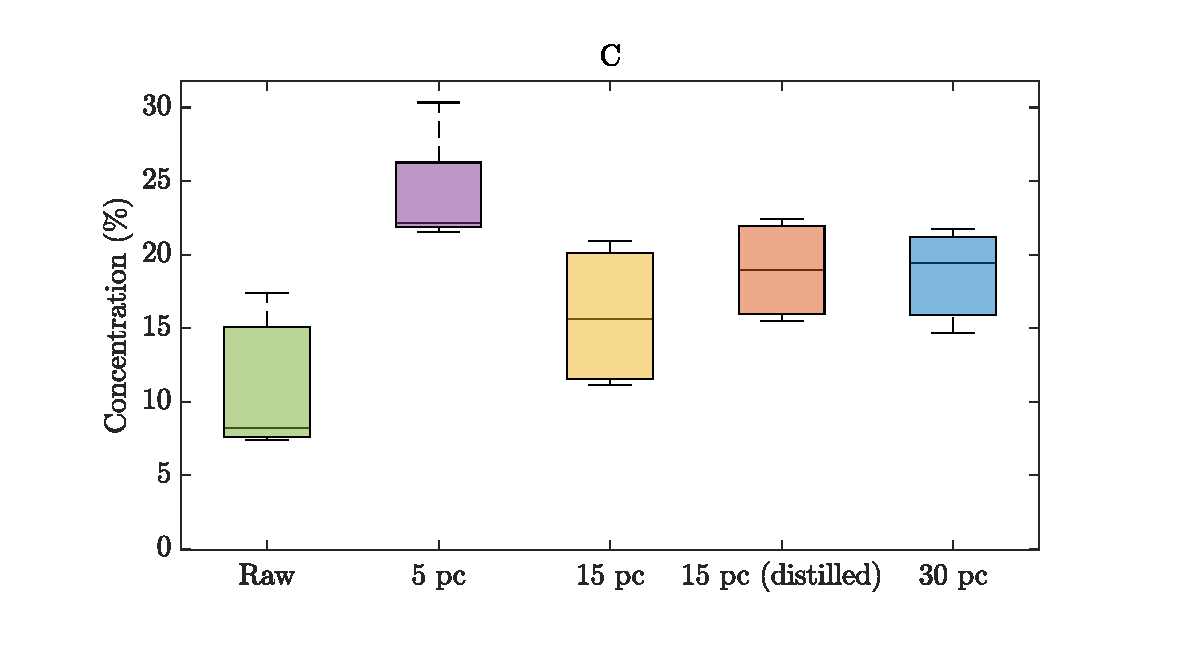
\includegraphics[width = \textwidth]{chapter_5/others/XPS/XPS_C_conc.pdf} 
   \vspace*{-30pt}
   \caption{Carbon concentration measured by XPS. }
   \label{fig:c_xps}
\end{figure}
The main carbon peak in LIBS is at $165 \: nm$, outside the range of our detector. For this reason the use of XPS to measure the concentration of this element was particularly important.
\\
Figure~\ref{fig:c_xps} shows a concentration of carbon both in the raw and the polished samples. The presence of carbonaceous compounds on the surfaces of the raw sample was already partially confirmed by the FTIR analysis in the form of a \ce{C-O} absorption peak (Chapter~\ref{sec:ftir_results}), while no traces were found in the ground and polished samples with the same technique. This could suggest that the nature of the carbon contaminants found on the raw and processed glass surfaces are different.
\\
Regarding chemical shift, here are presented the comparison between peaks of different samples:

\begin{figure}[H]
   \centering
   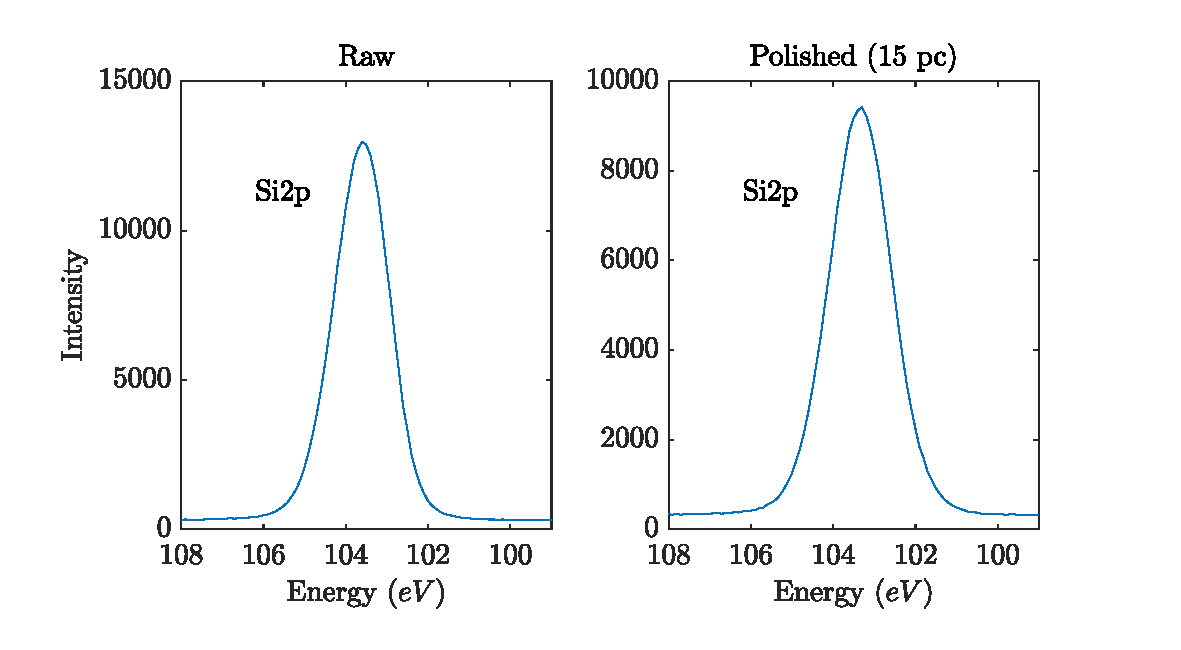
\includegraphics[width = \textwidth]{chapter_5/others/XPS/xps_chem_shift_si.pdf} 
   \vspace*{-30pt}
   \caption{Comparison of the \ce{Si}2p level measured with XPS. (Left) Raw sample. (Right) Polished sample.}
   \label{fig:xps_shift_si}
\end{figure}

\begin{figure}[H]
   \centering
   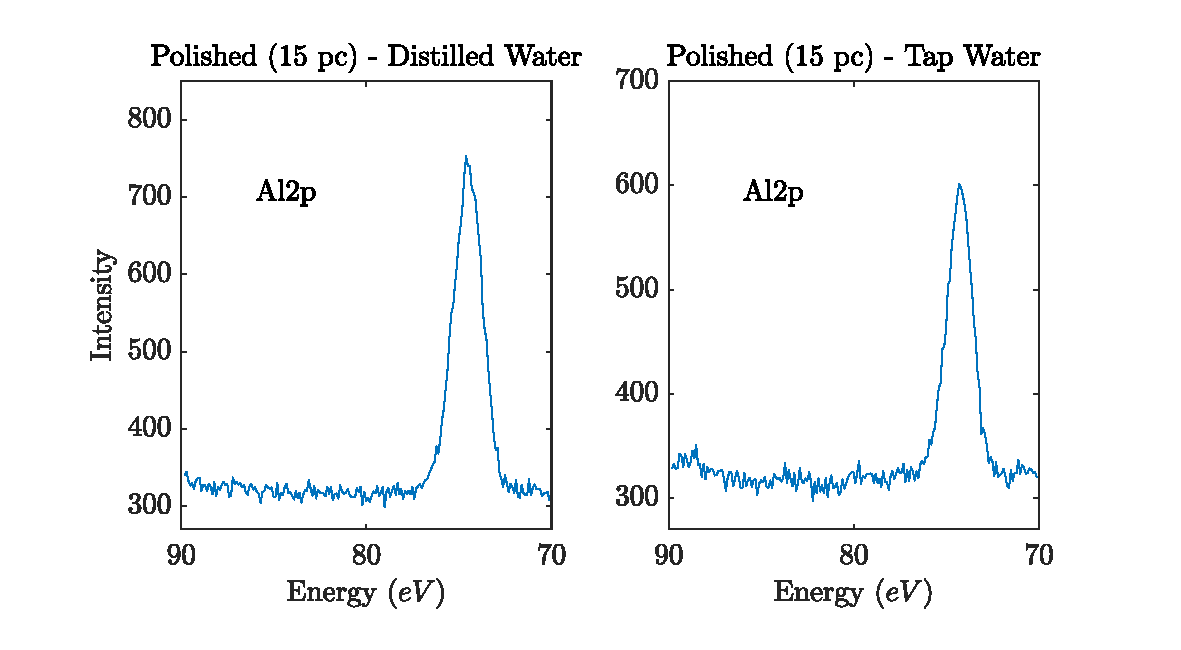
\includegraphics[width = \textwidth]{chapter_5/others/XPS/xps_chem_shift_al.pdf} 
   \vspace*{-30pt}
   \caption{Comparison of the \ce{Al}2p level measured with XPS. (Left) Polished with distilled water. (Right) Polished with tap water.}
   \label{fig:xps_shift_al}
\end{figure}

For what regards these elements, no new peak caused by chemical shift has been found.


\begin{figure}[H]
   \centering
   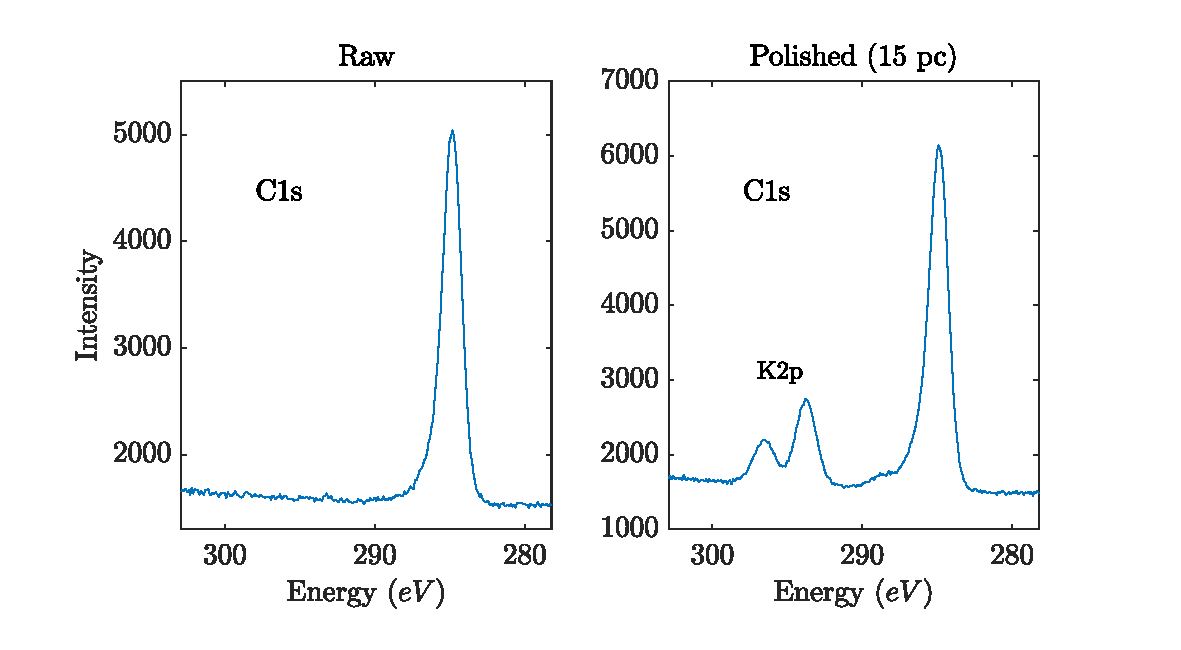
\includegraphics[width = \textwidth]{chapter_5/others/XPS/xps_chem_shift_c_corrected.pdf} 
   \vspace*{-30pt}
   \caption{Comparison of the \ce{C}1s level measured with XPS. (Left) Raw sample. (Right) Polished sample.}
   \label{fig:xps_shift_c}
\end{figure}

In Figure~\ref{fig:xps_shift_c} are present peaks that could be associated with the effect of chemical shift, however, a more probable explanation is the presence of potassium on the sample. This is because the chemical shift corresponding to those energies is associated with \ce{C-F} bonds, nonetheless, no traces of fluorine have been found from any analysis we performed.

In Figure~\ref{fig:xps_shift_c} at first glance the presence of chemically shifted carbon peaks could be implied. However, in that energy range, the peaks associated with the 2p level of potassium are found.
\section{LIBS}
\label{sec:LIBS_measurements}

In this section are presented the experimental results of the LIBS measurements, as well as the fitting to the theoretical concentrations.
\subsection{Data Fitting Method}
\label{subsec:data_fitting}
As already explained in detail in Chapter~\ref{sec:theoretical_prediction}, if normal diffusion is the primary driving mechanism for the presence of contaminants in the glass, the expected concentration of contaminants should follow Equation~\ref{eq:c_bar_equation}.
\\
In the expression there are three different parameters that can influence the behavior of the function: $d_a$, $C_0$ and $D$. They are, respectively, the ablation depth of the LIBS measurement, the saturation concentration and the diffusion constant.
\\
The ablation depth should be the same for every measurement we performed, as it only depends on the laser parameters and on the target material, both of which were constant for all the experiments.
\\
To estimate this parameter we have performed some depth analyses with a 3D microscope to a pure silica sample that was ablated five different times with the same laser energy of $15 \: mJ$ but with an increasing number of pulses, from 5 to 25.

\begin{figure}[H]
    \centering
    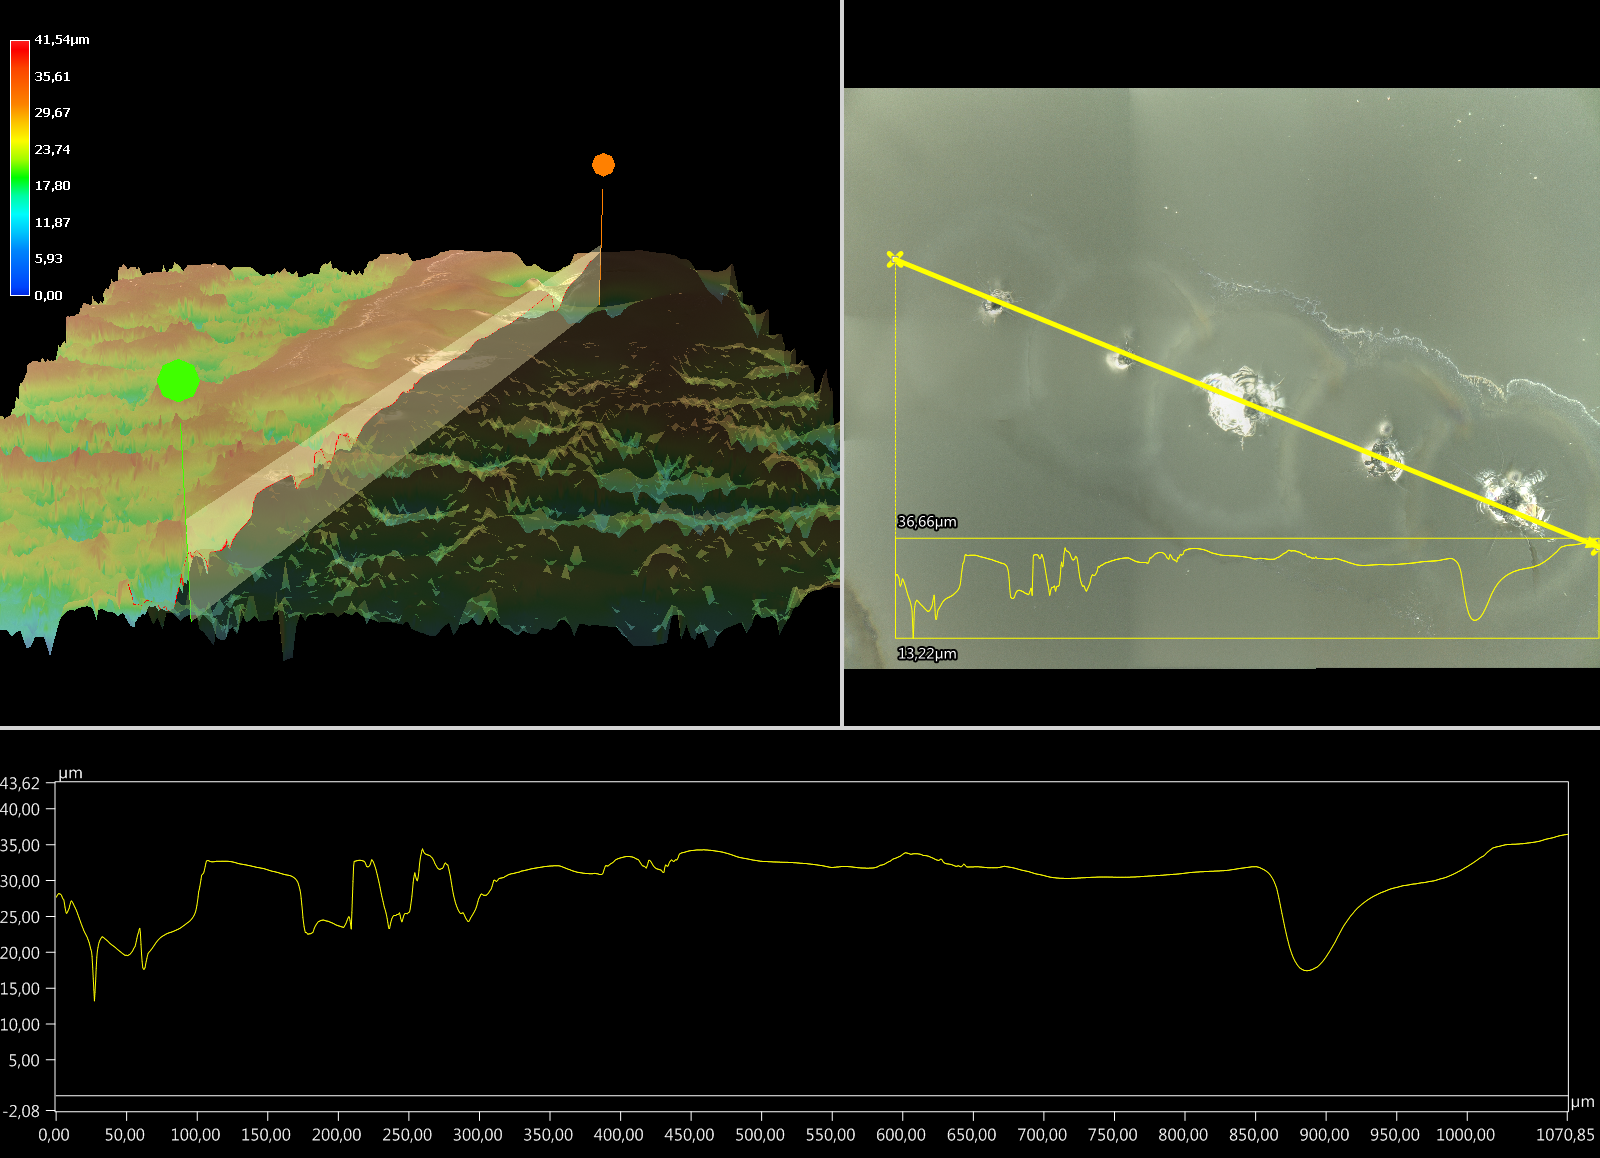
\includegraphics[width = 0.8\textwidth]{chapter_5/LIBS/data_fit/3dmicroscope_profile.png} 
    \caption{Width and depth measurements of LIBS craters performed with a 3D microscope. The peaks are ordered from left to right accordingly to the number of pulses.}
    \label{fig:3d_microscope_craters}
 \end{figure}

 Unfortunately, due to the translucency of silica glass, optical measuring methods cannot be fully trusted, especially when performing depth profiling. The information presented in Figure~\ref{fig:3d_microscope_craters} is only useful to give an idea of the order or magnitude of the value.
 \\
For the first two peaks, the ones corresponding to 5 and 10 pulses, the depth measured by the microscope is around $5 \: \mu m$. In the case of our experiments the energy was the same but only one pulse was performed, with consequently less ablation. As an estimation of the crater depth, we considered the value cited before but one order of magnitude lower, $d_a = 0.5 \: \mu m$.
\\
The two other parameters, $C_0$ and $D$, strictly depend on the specific characteristics of the diffusion.
\\
The of magnitude for $D$ in glasses can be found in literature; in [paper aluminum in glass] there is an estimation of the diffusion coefficient of gaseous metallic aluminum into the amorphous silica layer that forms on top of silicon wafers. The value is given by the following equation:
\begin{align}
    D/m^2s^{-1} = 1.83 \cdot 10^{-13}\exp \left(\frac{-1.12 \cdot 10^5}{RT}\right) \label{eq:diffiusion_coef_aluminum}
\end{align}
Where $R$ is the ideal gas constant and $T$ is the absolute temperature of the chamber. This expression is valid for values of the temperature between 973 and $1173 \:K$. By taking the middle value of that range, the corresponding $D$ is equal to $2.02 \cdot 10^{-18} \:m^2s^{-1}$.
\\
Regarding $C_0$, for the fitting procedure to make sense, the value of the parameter should be of the order of the experimental values; ideally, if the measurements follow a curve similar to the one in Figure~\ref{fig:c_bar_mixed}, the value of $C_0$ should be the one corresponding to the concentrations of the values taken at later polishing times.
\\
For the actual fitting, we employed a simple algorithm. We defined two arrays with the possible values of $D$ and $C_0$: for $D$ we constructed a logarithmic space between $10^{-20}$ and $10^{-7}$, while for $C_0$ we built a linear space between the minimum and two times the maximum the measured concentration of the element we were trying to fit.
\\
We then constructed another array with all the possible combinations between the two parameters, and, finally, we identified the couple that resulted in the least round mean square (rms) of the difference between the theoretical function and the data.
\\
The whole procedure should be enough to perform qualitative comparisons between different species.





\subsection{Concentration of the Polishing Solution}
\label{subsec:conc_results}
In the next section we will display all the collected data. Initially, for each polish concentration, a qualitative comparison of the notable wavelength ranges between the spectra of the raw, ground and polished sample is shown. Secondly, the plots with the measured contaminants concentrations are presented. The diffusion parameters fitted with the method proposed in the previous section are also shown. Lastly, we will exhibit the differences between the measured contaminants relatively to the polish suspension concentration.
\\
The solutions with different concentrations and water types were also distinguished by a different level of pH, in Table~\ref{table:solution_ph} are shown the corresponding value. The values were all measured using litmus paper.

\begin{table}[H]
   \centering
   \begin{tabular}{lclll}
   \hline
   \multicolumn{1}{|c|}{Water Type} & \multicolumn{1}{c|}{Pure} & \multicolumn{1}{c|}{5pc}   & \multicolumn{1}{c|}{15pc}  & \multicolumn{1}{c|}{30pc} \\ \hline
   \multicolumn{1}{|c|}{Tap}        & \multicolumn{1}{c|}{6,5}  & \multicolumn{1}{c|}{6,5-7} & \multicolumn{1}{c|}{8-8,5} & \multicolumn{1}{c|}{9}    \\ \hline
   \multicolumn{1}{|c|}{Distilled}  & \multicolumn{1}{c|}{6}    & \multicolumn{1}{c|}{-}     & \multicolumn{1}{c|}{9}     & \multicolumn{1}{c|}{-}    \\ \hline
   \end{tabular}
   \caption{pH level of the polishing solutions relative to the concentration and type of water.}
        \label{table:solution_ph}
   \end{table}
\subsubsection{Polish Concentration: 5pc}
\label{subsubsec:5pc}
\vspace*{-25pt}
\begin{figure}[H]
    \centering
    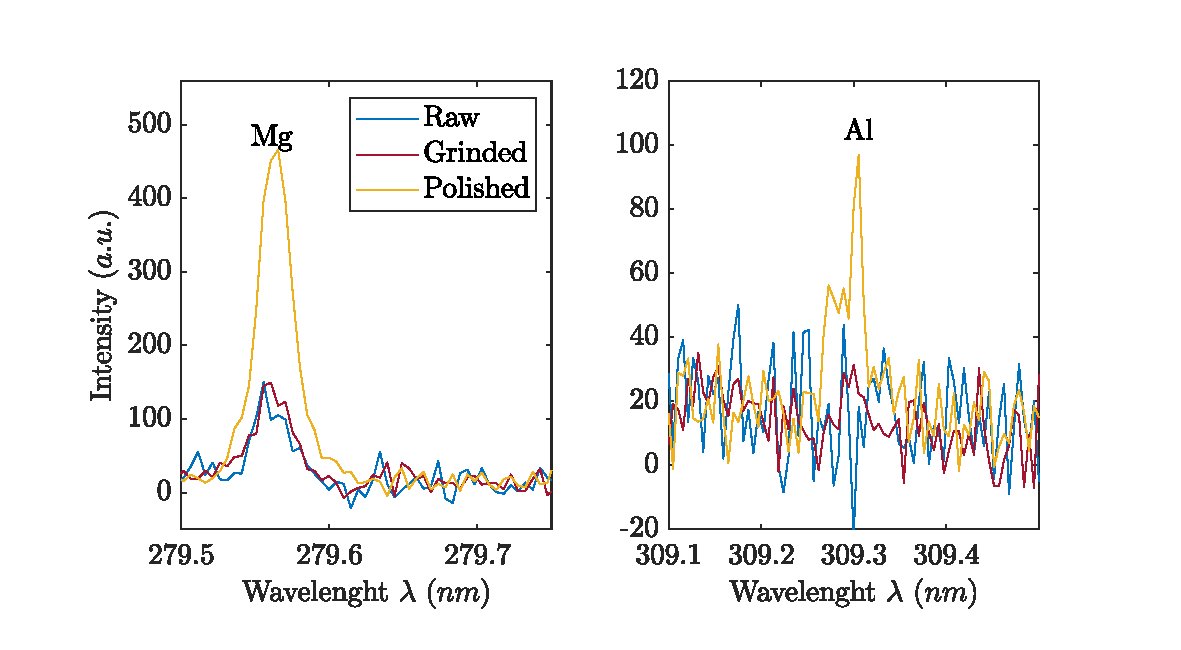
\includegraphics[width = \textwidth]{chapter_5/LIBS/spectra_comparison/tap_5pc_first.pdf} 
    %\caption{Width and depth measurements of LIBS craters performed with a 3D microscope. The peaks are ordered from left to right accordingly to the number of pulses.}
    %\label{fig:3d_microscope_craters}
 \end{figure}

\vspace*{-68pt}
\begin{figure}[H]
    \centering
    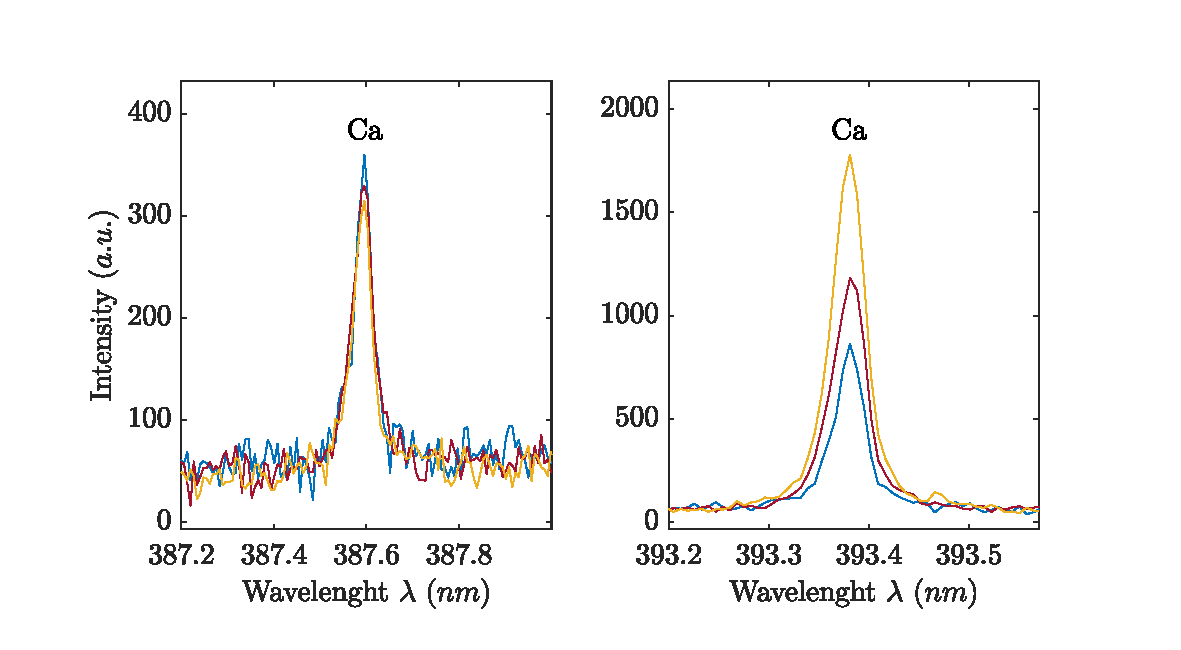
\includegraphics[width = \textwidth]{chapter_5/LIBS/spectra_comparison/tap_5pc_second.pdf} 
    %\caption{Width and depth measurements of LIBS craters performed with a 3D microscope. The peaks are ordered from left to right accordingly to the number of pulses.}
    %\label{fig:3d_microscope_craters}
 \end{figure}

\vspace*{-68pt}
\begin{figure}[H]
    \centering
    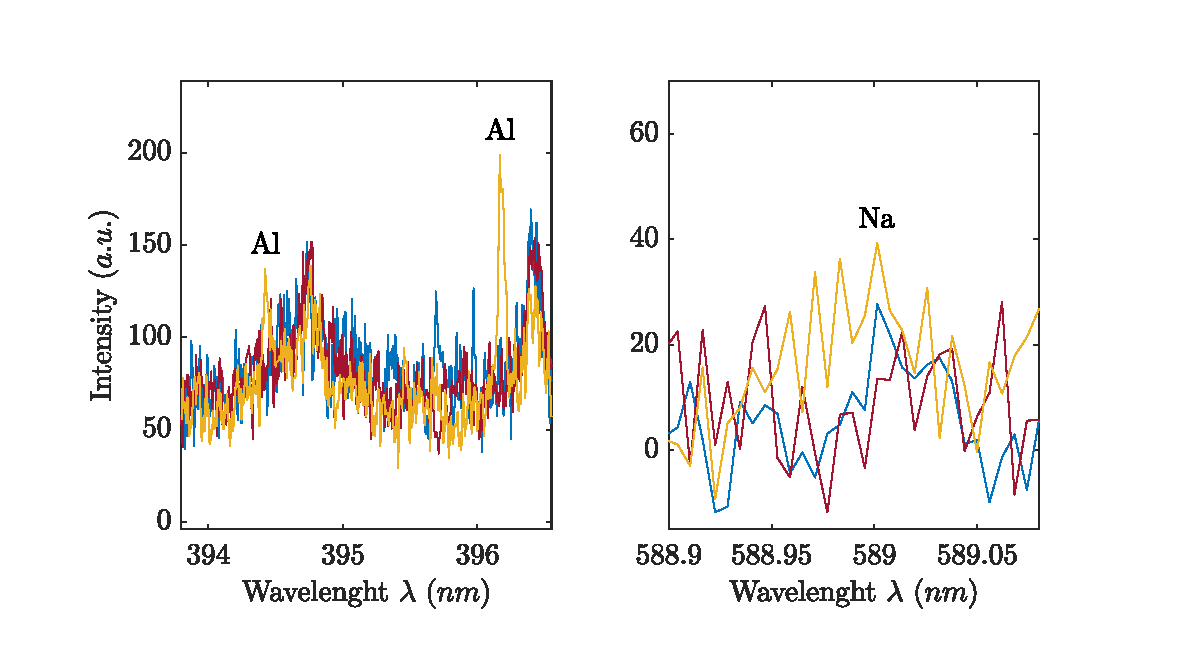
\includegraphics[width = \textwidth]{chapter_5/LIBS/spectra_comparison/tap_5pc_third.pdf} 
    %\caption{Width and depth measurements of LIBS craters performed with a 3D microscope. The peaks are ordered from left to right accordingly to the number of pulses.}
    %\label{fig:3d_microscope_craters}
 \end{figure}

 As it can be seen from the plots, the polished sample can be easily distinguished from the other two spectra; in particular, the aluminum peaks are present only in the polished sampled, while the other elements are found also in the raw and ground spectra. Due to the lower sensitivity of the detector in the visible range, the sodium peak cannot be easily distinguished from the noise floor. Its presence is expected since, as shown in Table~\ref{table:water_composition}, a non-negligible quantity is dissolved in the water. Moreover, sodium has a low LOD and should be easily detectable with LIBS.
\\
For the next series of graphs, only the time evolution of the polishing phase is shown.
\begin{figure}[H]
    \centering
    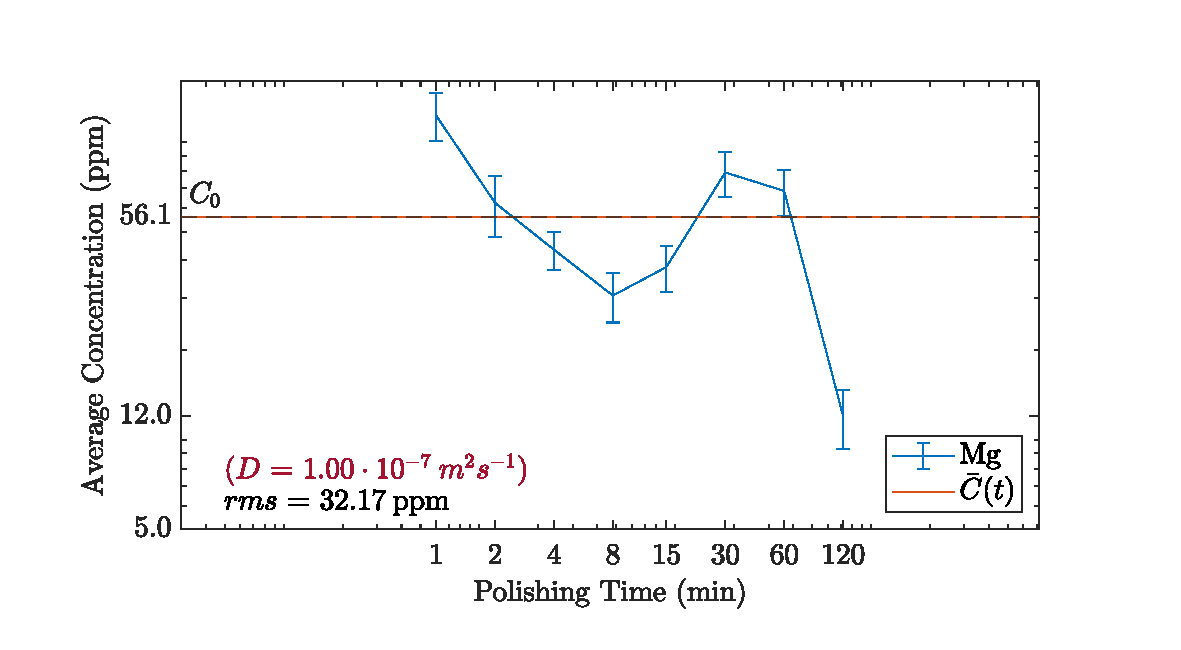
\includegraphics[width = \textwidth]{chapter_5/LIBS/data_fit/fit_tap_5pc_Mg.pdf} 
    %\caption{Width and depth measurements of LIBS craters performed with a 3D microscope. The peaks are ordered from left to right accordingly to the number of pulses.}
    %\label{fig:3d_microscope_craters}
 \end{figure}
\vspace*{-48pt}
 \begin{figure}[H]
    \centering
    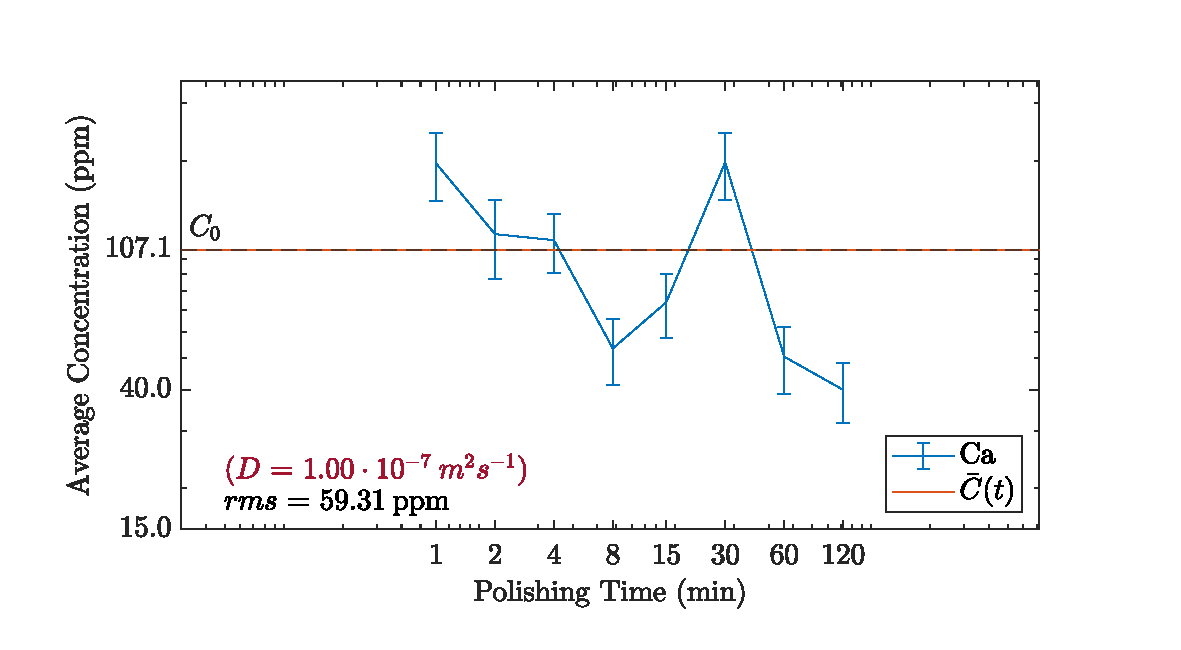
\includegraphics[width = \textwidth]{chapter_5/LIBS/data_fit/fit_tap_5pc_Ca.pdf} 
    %\caption{Width and depth measurements of LIBS craters performed with a 3D microscope. The peaks are ordered from left to right accordingly to the number of pulses.}
    %\label{fig:3d_microscope_craters}
 \end{figure}
 \begin{figure}[H]
    \centering
    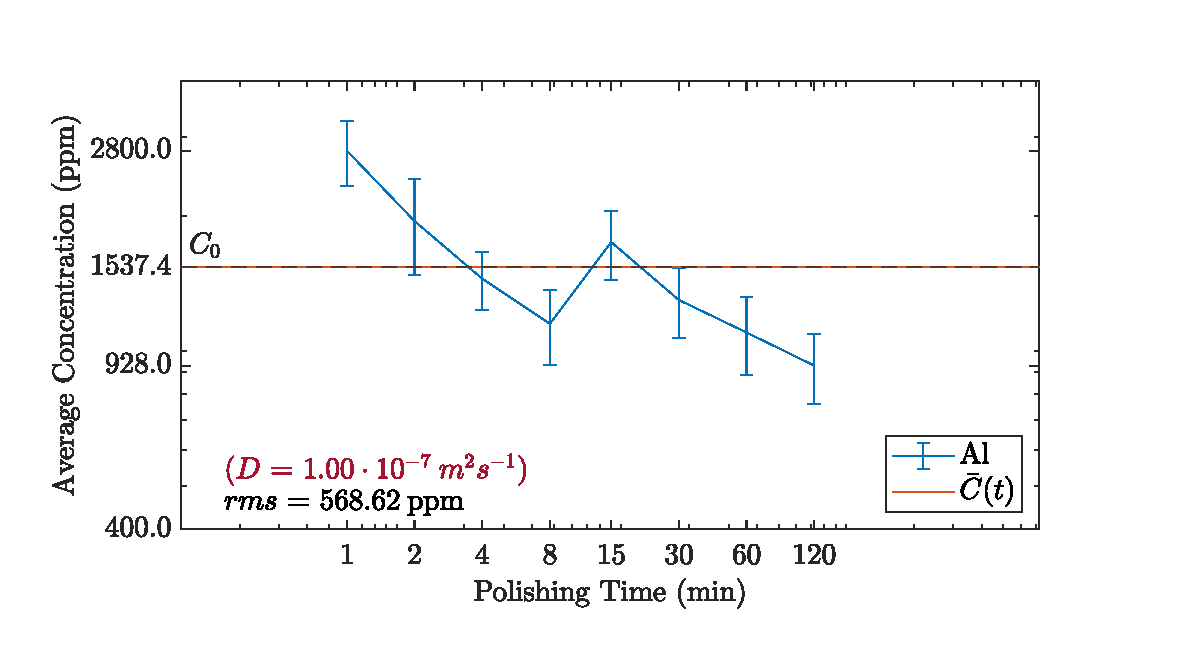
\includegraphics[width = \textwidth]{chapter_5/LIBS/data_fit/fit_tap_5pc_Al.pdf} 
    %\caption{Width and depth measurements of LIBS craters performed with a 3D microscope. The peaks are ordered from left to right accordingly to the number of pulses.}
    %\label{fig:3d_microscope_craters}
 \end{figure}

    \vspace*{-20pt}
 \begin{figure}[H]
    \centering
    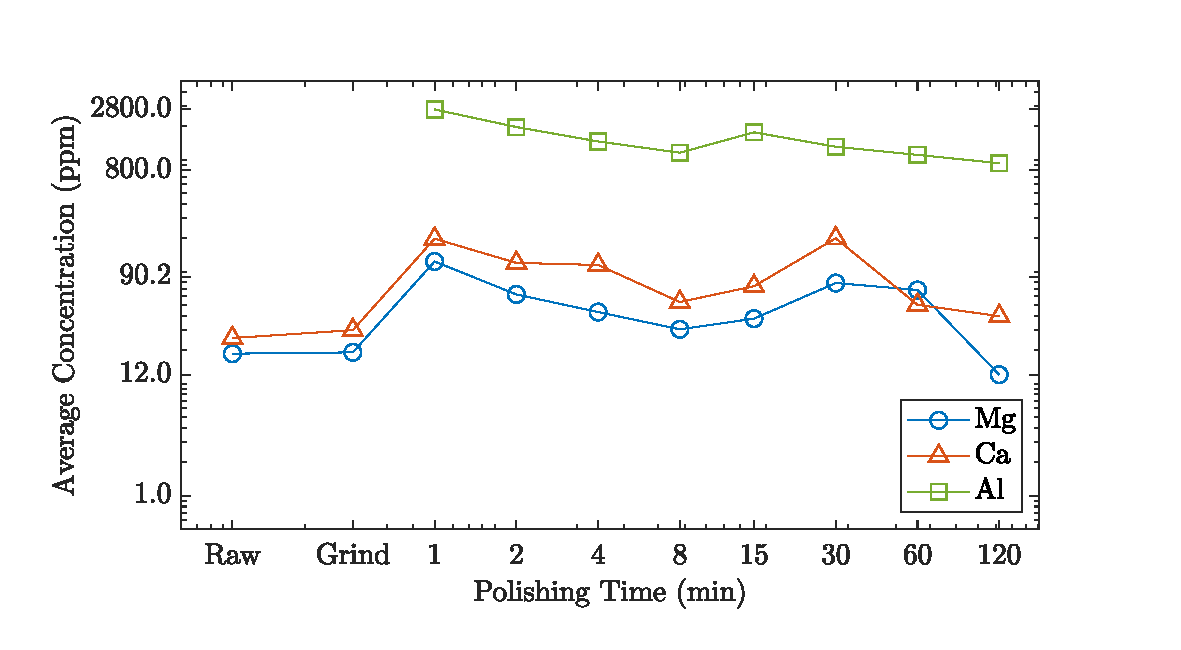
\includegraphics[width = \textwidth]{chapter_5/LIBS/Tap_elem_comparisons/Tap_elements_5_pc.pdf} 
    \vspace*{-30pt}
    \caption{Comparison of the concentration values of the major contaminants as a function of the polishing time, for the glass polished with a 5pc suspension.}
    \label{fig:tap_elem_5pc}
 \end{figure}
 In Figure~\ref{fig:tap_elem_5pc} it is clear that all the elements share a similar decreasing behavior.





\pagebreak



\subsubsection{Polish Concentration: 15pc}
\label{subsubsec:15pc}
\vspace*{-25pt}
\begin{figure}[H]
    \centering
    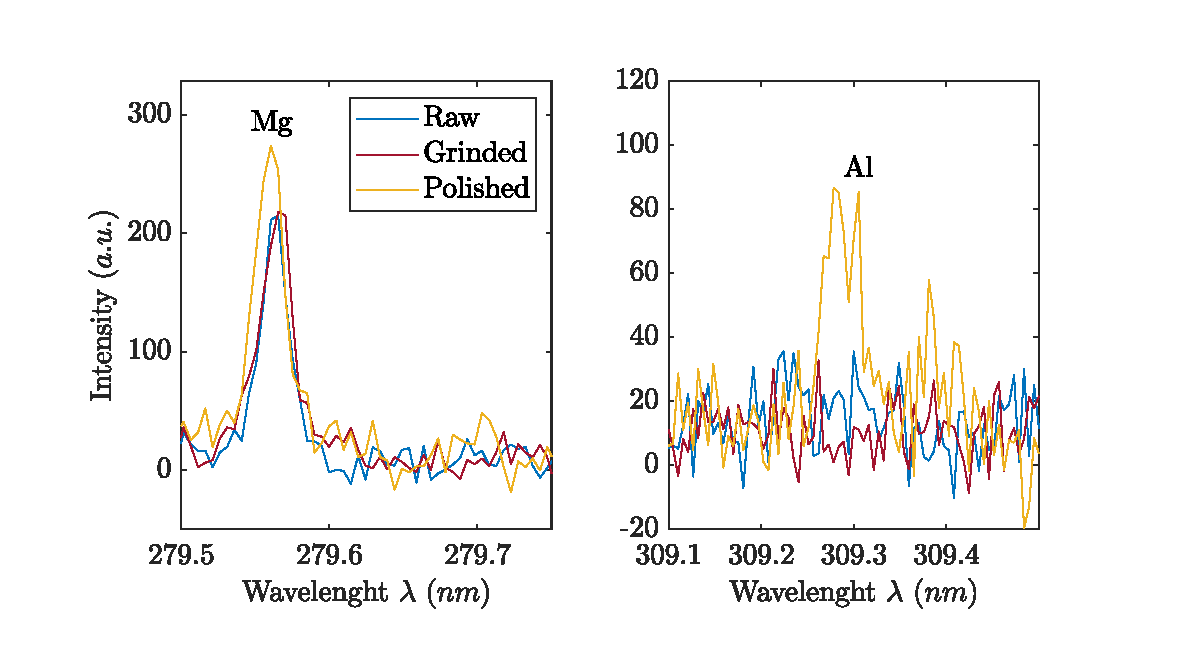
\includegraphics[width = \textwidth]{chapter_5/LIBS/spectra_comparison/tap_15pc_first.pdf} 
    %\caption{Width and depth measurements of LIBS craters performed with a 3D microscope. The peaks are ordered from left to right accordingly to the number of pulses.}
    %\label{fig:3d_microscope_craters}
 \end{figure}

\vspace*{-68pt}
\begin{figure}[H]
    \centering
    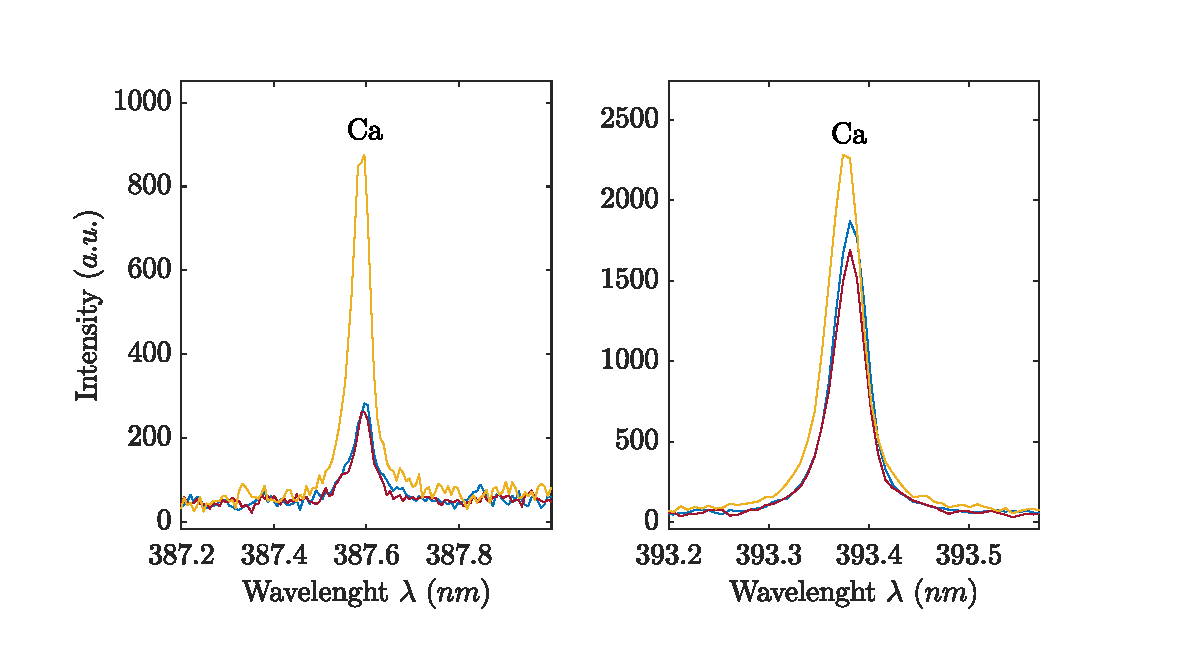
\includegraphics[width = \textwidth]{chapter_5/LIBS/spectra_comparison/tap_15pc_second.pdf} 
    %\caption{Width and depth measurements of LIBS craters performed with a 3D microscope. The peaks are ordered from left to right accordingly to the number of pulses.}
    %\label{fig:3d_microscope_craters}
 \end{figure}

\vspace*{-68pt}
\begin{figure}[H]
    \centering
    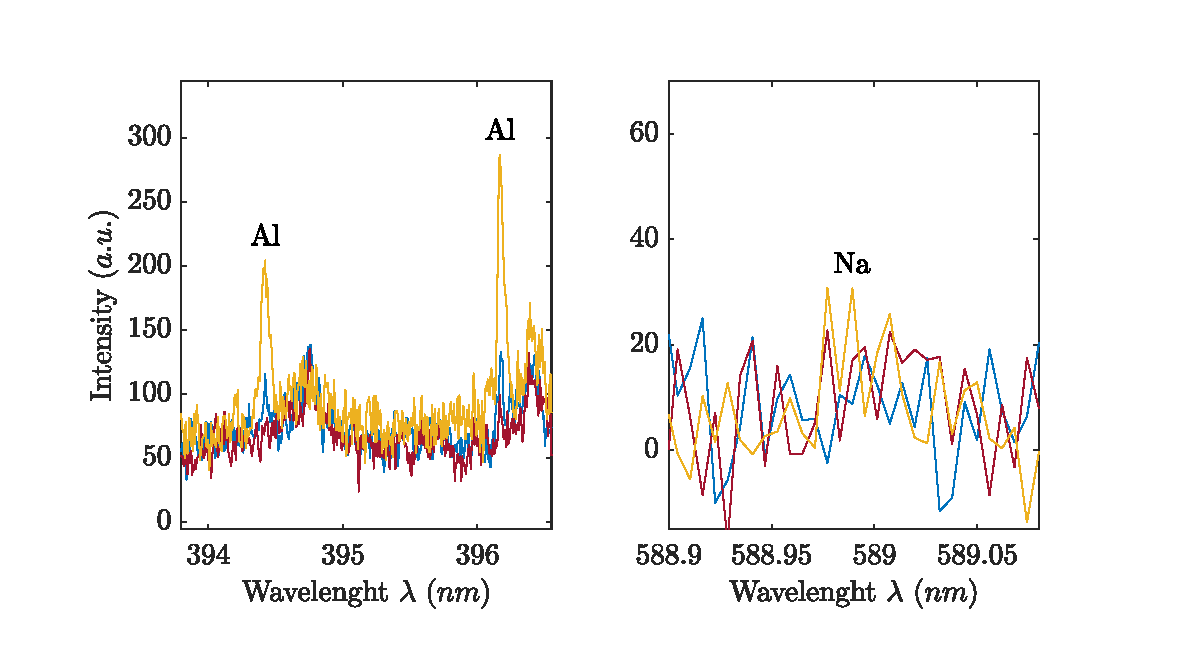
\includegraphics[width = \textwidth]{chapter_5/LIBS/spectra_comparison/tap_15pc_third.pdf} 
    %\caption{Width and depth measurements of LIBS craters performed with a 3D microscope. The peaks are ordered from left to right accordingly to the number of pulses.}
    %\label{fig:3d_microscope_craters}
 \end{figure}

 The behavior of the spectra is similar to the 5pc case. The most notable difference is the in the \ce{Ca} peaks, where in this case, the difference between the polished and unpolished sample is more relevant in the peak located at a  smaller wavelength. This could probably be related to differences in the characteristics of the plasma, like temperature and electron density.

\begin{figure}[H]
    \centering
    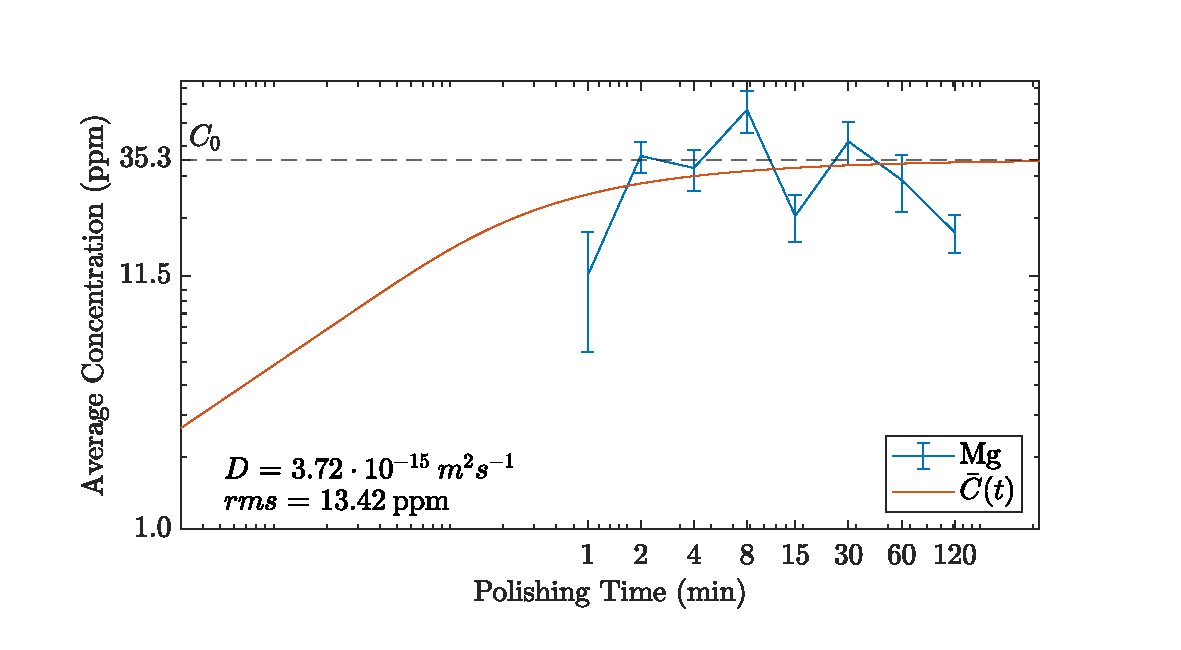
\includegraphics[width = \textwidth]{chapter_5/LIBS/data_fit/fit_tap_15pc_Mg.pdf} 
    \vspace{-30pt}
    \caption{Measurement for the Mg concentration fitted to the diffusion model.}
    \label{fig:fit_tap_15pc}
 \end{figure}

 \begin{figure}[H]
    \centering
    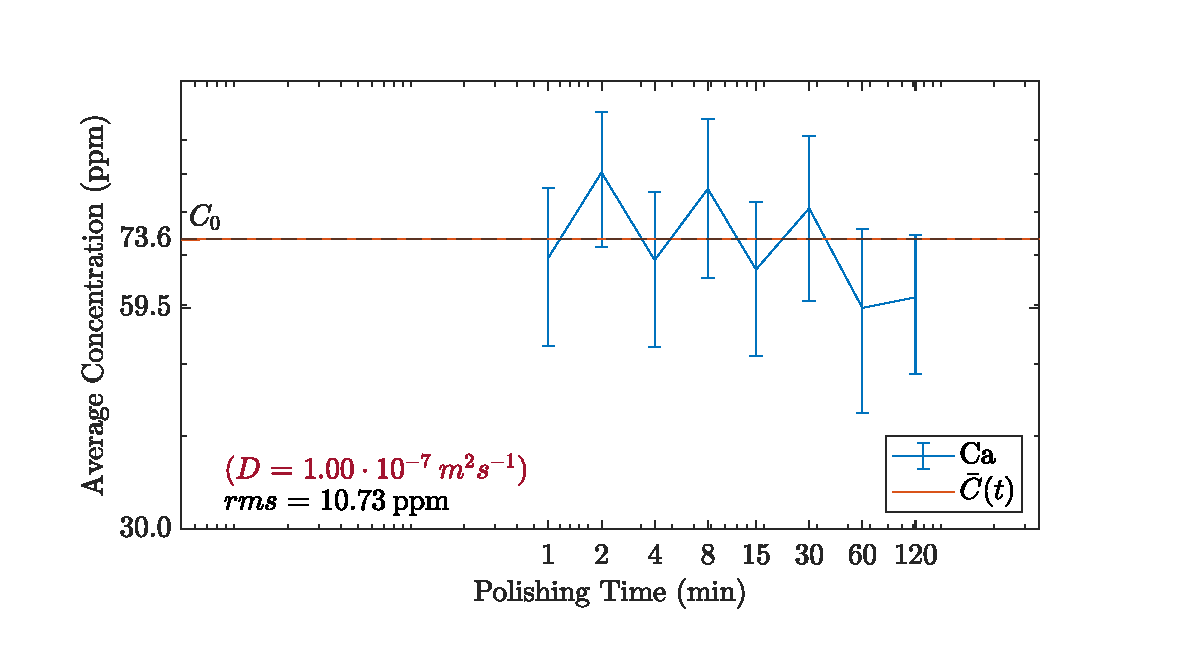
\includegraphics[width = \textwidth]{chapter_5/LIBS/data_fit/fit_tap_15pc_Ca.pdf} 
    %\caption{Width and depth measurements of LIBS craters performed with a 3D microscope. The peaks are ordered from left to right accordingly to the number of pulses.}
    %\label{fig:3d_microscope_craters}
 \end{figure}
    \vspace{-40pt}
 \begin{figure}[H]
    \centering
    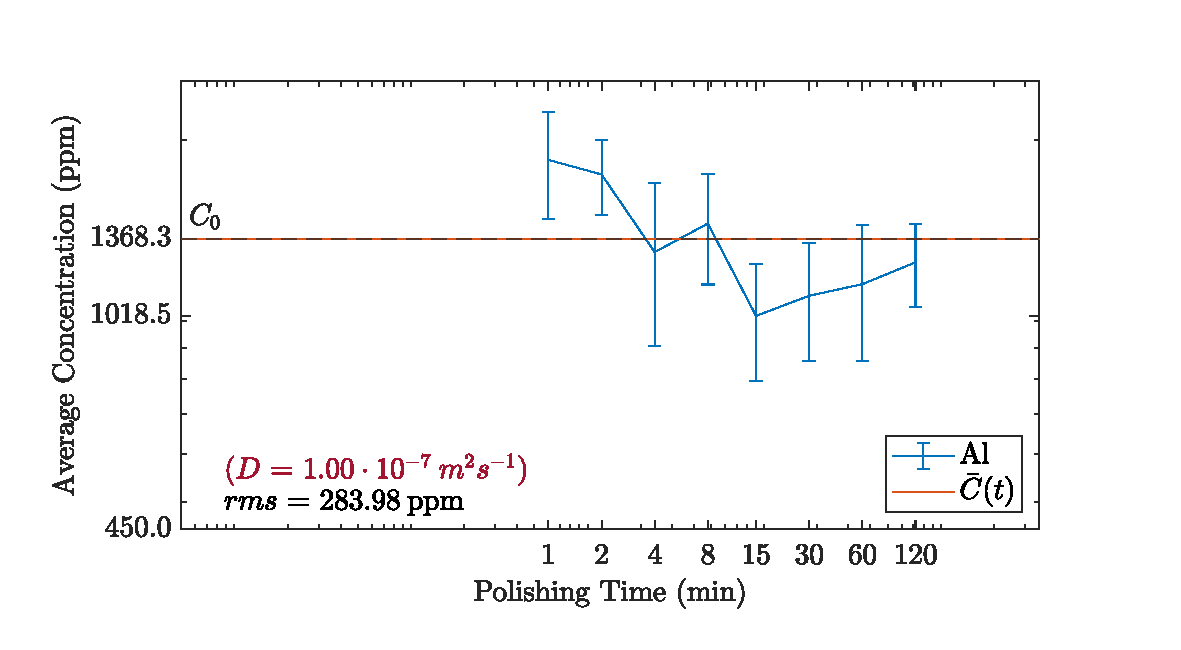
\includegraphics[width = \textwidth]{chapter_5/LIBS/data_fit/fit_tap_15pc_Al.pdf} 
    %\caption{Width and depth measurements of LIBS craters performed with a 3D microscope. The peaks are ordered from left to right accordingly to the number of pulses.}
    %\label{fig:3d_microscope_craters}
 \end{figure}

 \vspace{-20pt}

 As can be seen from Figure~\ref{fig:fit_tap_15pc}, in this case, the data could be fairly fitted by the algorithm exposed in Chapter~\ref{subsec:data_fitting}. The diffusion coefficient estimated is much greater that the ones found in literature [cit acqua]. This could be caused by the value of $d_a$, that was heavily approximated. However, this set of data was the only one that had this result.

 \vspace{-20pt}
 \begin{figure}[H]
    \centering
    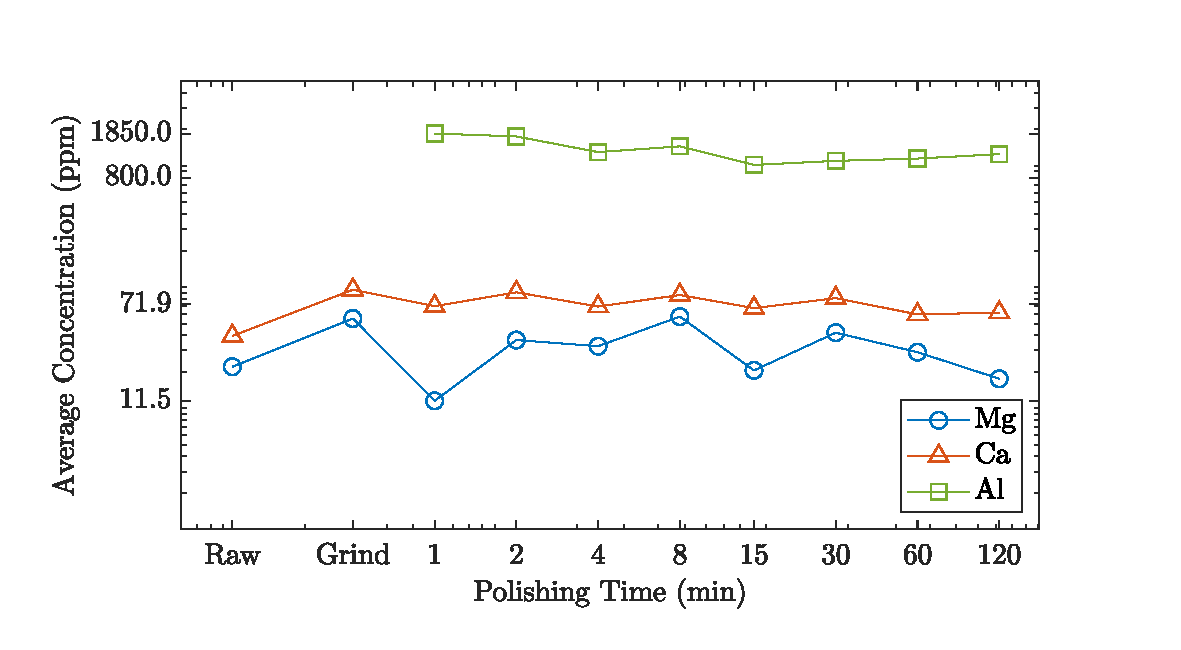
\includegraphics[width = \textwidth]{chapter_5/LIBS/Tap_elem_comparisons/Tap_elements_15_pc.pdf} 
    \vspace*{-30pt}
    \caption{Comparison of the concentration values of the major contaminants as a function of the polishing time, for the glass polished with a 15pc suspension.}
    \label{fig:tap_elem_15pc}
 \end{figure}

 The evolution of the concentrations of the elements is similar to the case presented in the previous section, with only slightly less variation.









 \subsubsection{Polish Concentration: 30pc}
 \label{subsubsec:30pc}
 \vspace*{-25pt}
 \begin{figure}[H]
     \centering
     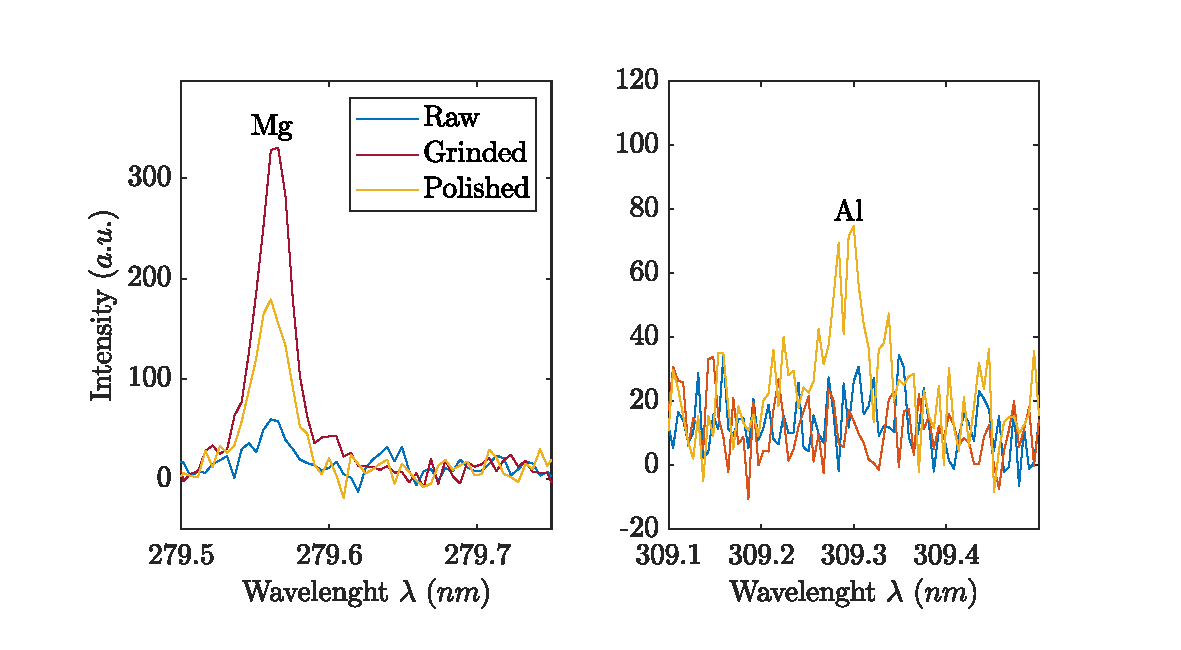
\includegraphics[width = \textwidth]{chapter_5/LIBS/spectra_comparison/tap_30pc_first.pdf} 
     %\caption{Width and depth measurements of LIBS craters performed with a 3D microscope. The peaks are ordered from left to right accordingly to the number of pulses.}
     %\label{fig:3d_microscope_craters}
  \end{figure}
 
 \vspace*{-68pt}
 \begin{figure}[H]
     \centering
     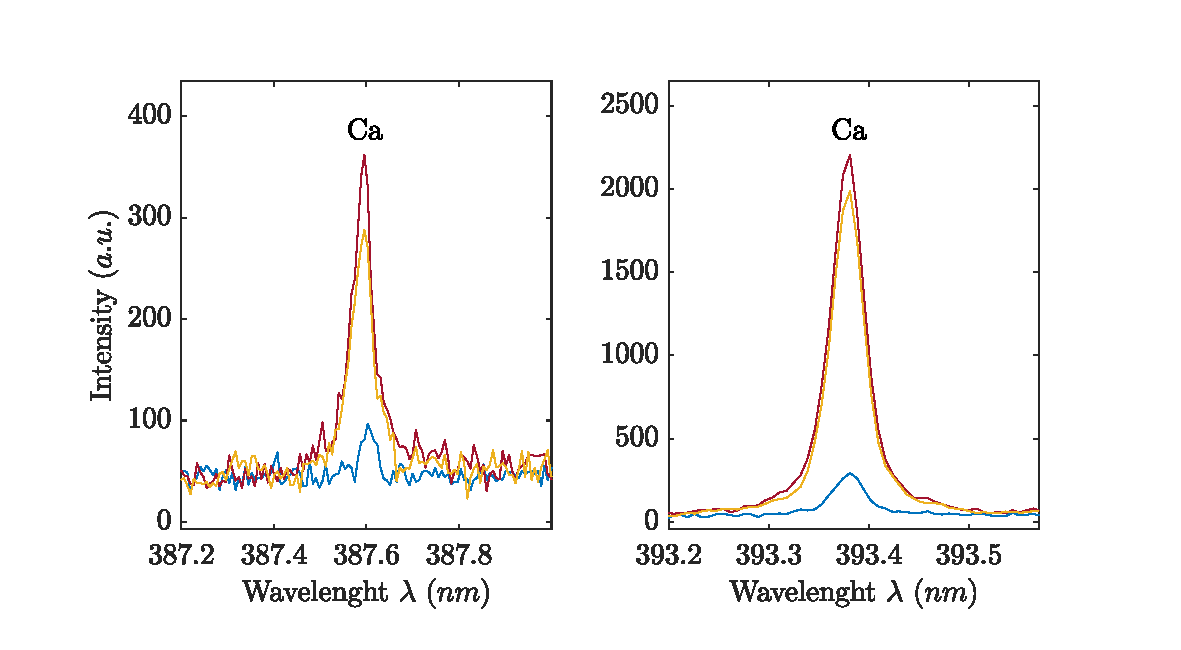
\includegraphics[width = \textwidth]{chapter_5/LIBS/spectra_comparison/tap_30pc_second.pdf} 
     %\caption{Width and depth measurements of LIBS craters performed with a 3D microscope. The peaks are ordered from left to right accordingly to the number of pulses.}
     %\label{fig:3d_microscope_craters}
  \end{figure}
 
 \vspace*{-68pt}
 \begin{figure}[H]
     \centering
     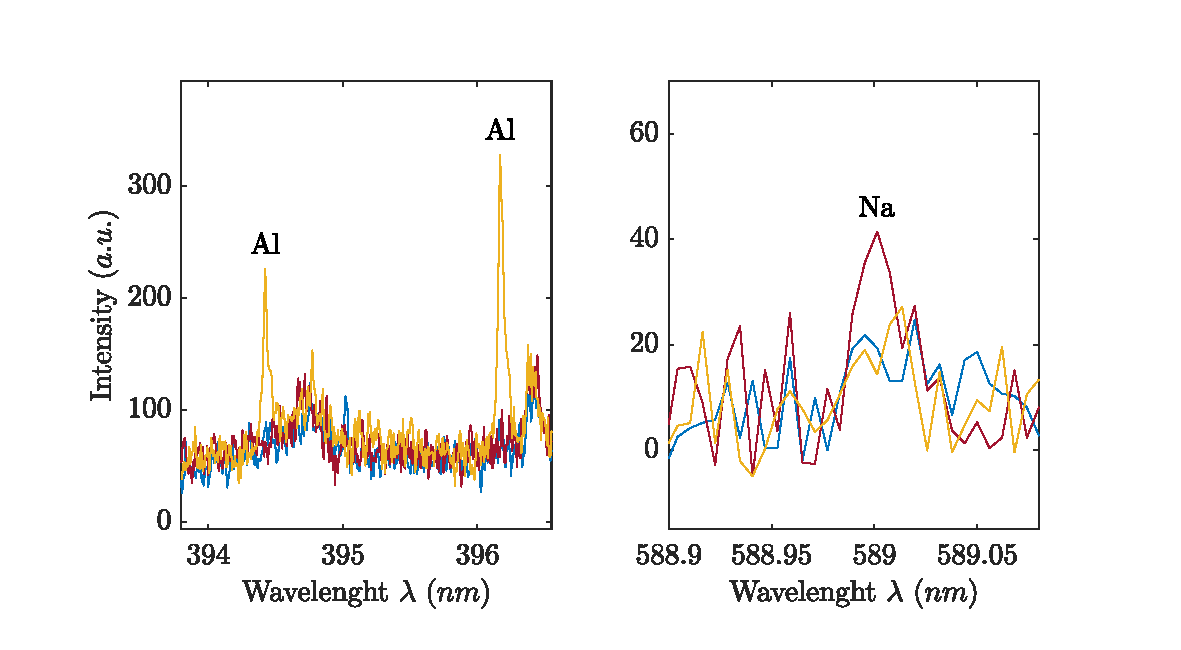
\includegraphics[width = \textwidth]{chapter_5/LIBS/spectra_comparison/tap_30pc_third.pdf} 
     %\caption{Width and depth measurements of LIBS craters performed with a 3D microscope. The peaks are ordered from left to right accordingly to the number of pulses.}
     %\label{fig:3d_microscope_craters}
  \end{figure}
 
From the magnesium and calcium plots, it appears that the concentration of water-related contaminants is much higher in the ground sample. This is confirmed from the Figure~\ref{fig:tap_elem_30pc}, where it is evident that the concentration of those elements is lower at the final stages of polishing.

 \begin{figure}[H]
     \centering
     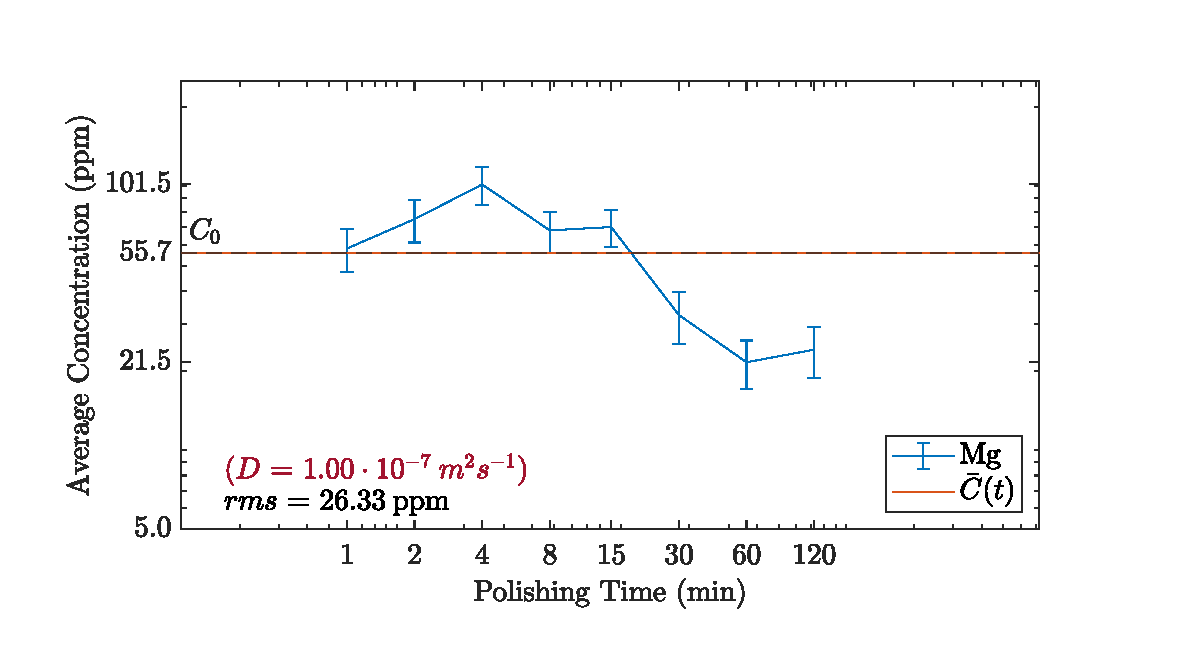
\includegraphics[width = \textwidth]{chapter_5/LIBS/data_fit/fit_tap_30pc_Mg.pdf} 
  \end{figure}
 
  \begin{figure}[H]
     \centering
     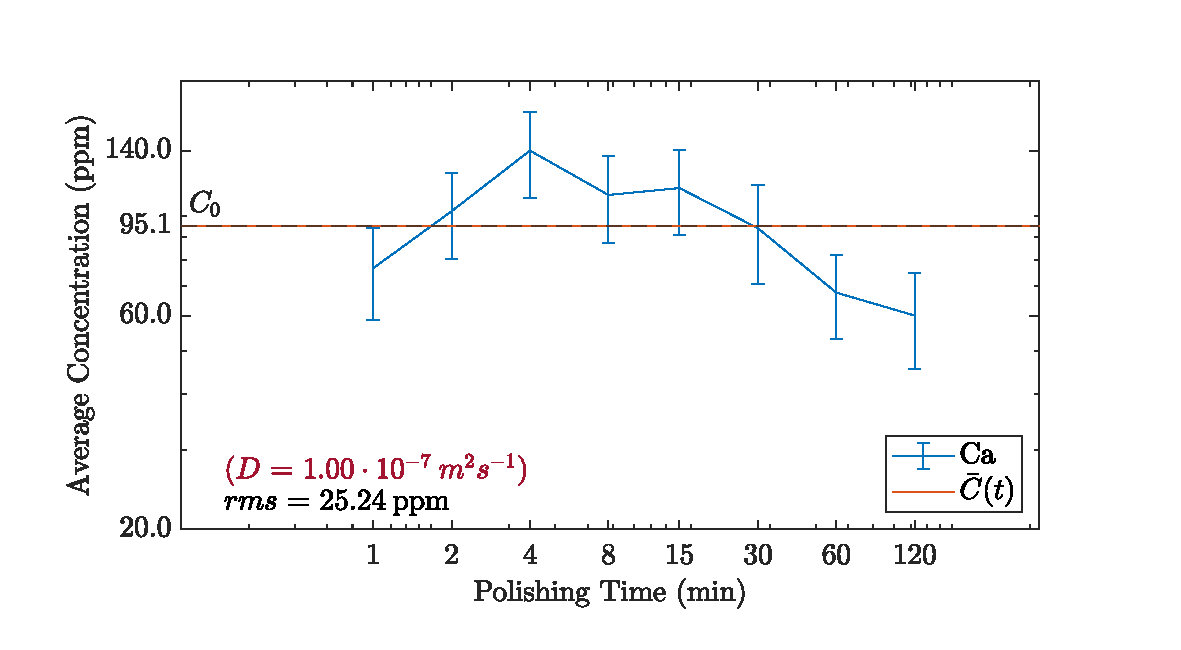
\includegraphics[width = \textwidth]{chapter_5/LIBS/data_fit/fit_tap_30pc_Ca.pdf} 
     %\caption{Width and depth measurements of LIBS craters performed with a 3D microscope. The peaks are ordered from left to right accordingly to the number of pulses.}
     %\label{fig:3d_microscope_craters}
  \end{figure}
     \vspace{-40pt}
  \begin{figure}[H]
     \centering
     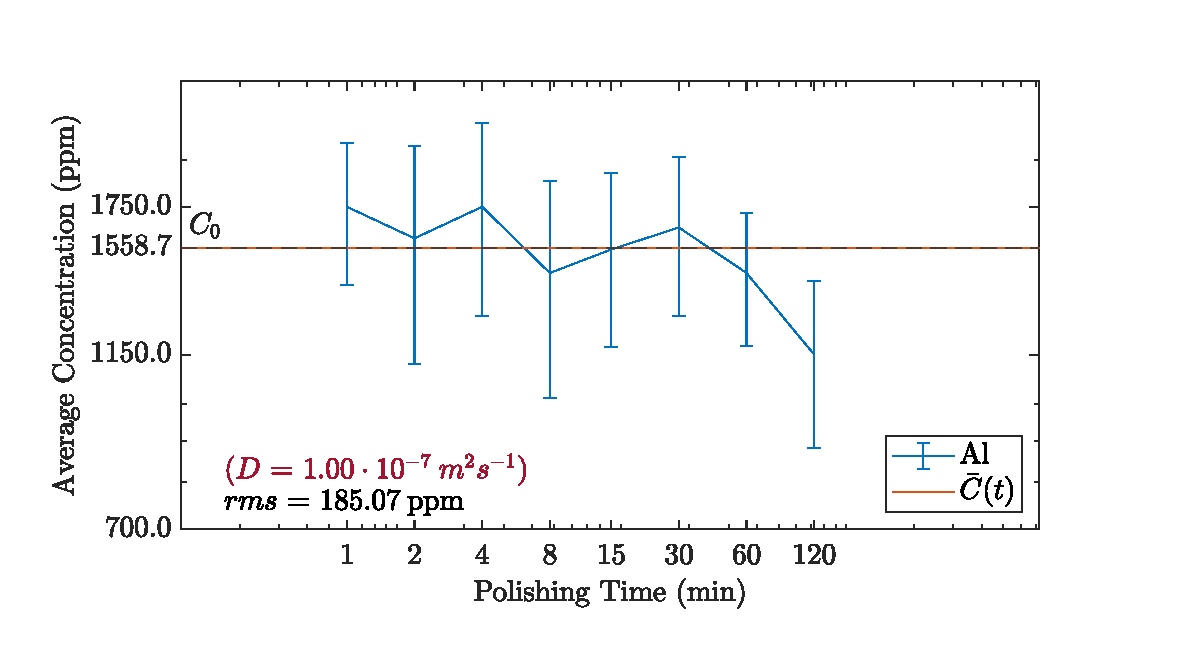
\includegraphics[width = \textwidth]{chapter_5/LIBS/data_fit/fit_tap_30pc_Al.pdf} 
     %\caption{Width and depth measurements of LIBS craters performed with a 3D microscope. The peaks are ordered from left to right accordingly to the number of pulses.}
     %\label{fig:3d_microscope_craters}
  \end{figure}

 
  \begin{figure}[H]
     \centering
     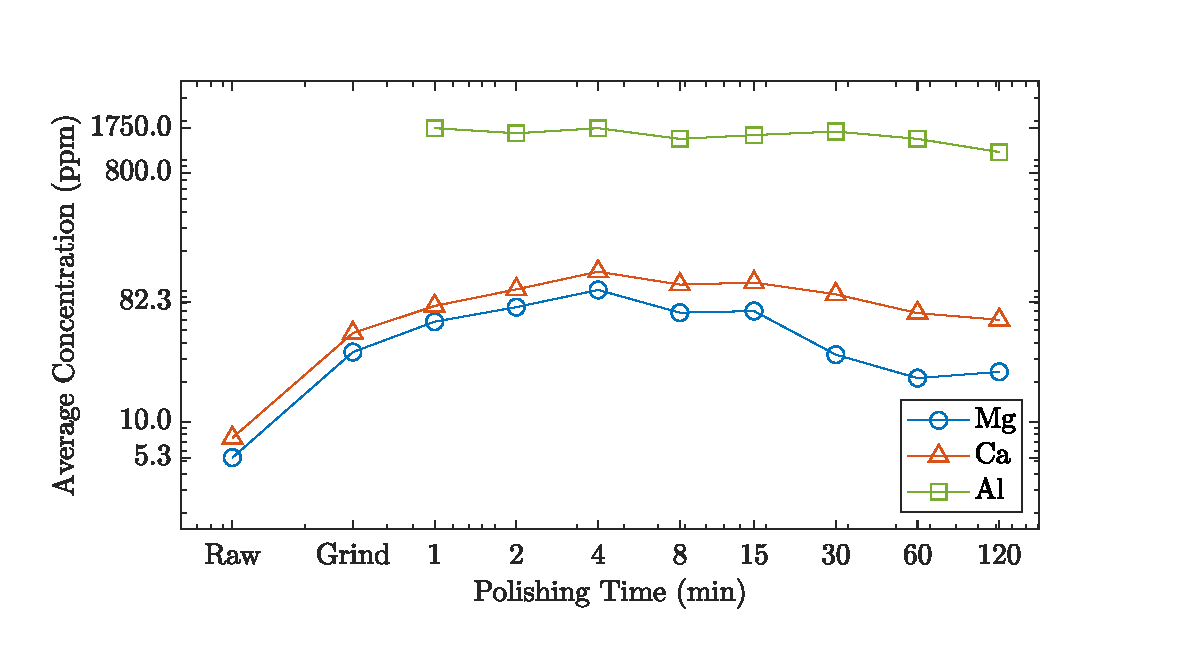
\includegraphics[width = \textwidth]{chapter_5/LIBS/Tap_elem_comparisons/Tap_elements_30_pc.pdf} 
     \vspace*{-30pt}
     \caption{Comparison of the concentration values of the major contaminants as a function of the polishing time, for the glass polished with a 30pc suspension.}
     \label{fig:tap_elem_30pc}
  \end{figure}


\subsubsection{Comparison between Polish Concentrations}
\label{subsubsec:comp_between_pol_conc}


\begin{figure}[H]
   \centering
   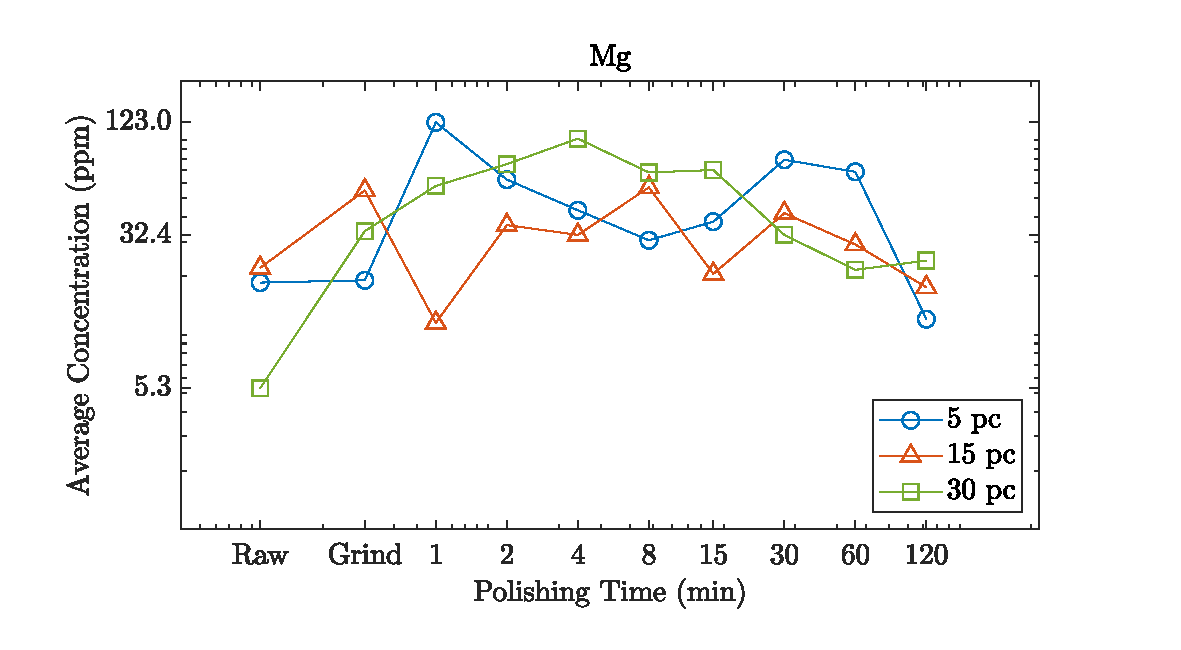
\includegraphics[width = \textwidth]{chapter_5/LIBS/Tap_conc_comparisons/Tap_conc_comp_Mg.pdf} 
   \vspace*{-30pt}
   \caption{Comparison between the magnesium concentrations relative to the different polishing solutions.}
   \label{fig:tap_conc_comp_mg}
\end{figure}

\begin{figure}[H]
   \centering
   \includegraphics[width = \textwidth]{chapter_5/LIBS/Tap_conc_comparisons/Tap_conc_comp_ca.pdf} 
   \vspace*{-30pt}
   \caption{Comparison between the calcium concentrations relative to the different polishing solutions.}
   \label{fig:tap_conc_comp_ca}
\end{figure}

\begin{figure}[H]
   \centering
   \includegraphics[width = \textwidth]{chapter_5/LIBS/Tap_conc_comparisons/Tap_conc_comp_al.pdf} 
   \vspace*{-30pt}
   \caption{Comparison between the aluminum concentrations relative to the different polishing solutions.}
   \label{fig:tap_conc_comp_al}
\end{figure}

The most notable consideration that can be derived from these graphs is that the presence of aluminum on the surface does not seem to have a clear dependence on the concentration of the solution. Moreover, the aluminum appears to have a more evident decreasing behavior respect to the other contaminants. 
%This could be partially related to the fact that alumina is not soluble, unlike, for example, calcium carbonate which should be the main cause of the presence of calcium.
%\\
%More details on this hypothesis will be presented in Chapter~\ref{sec:considerations}.

\subsection{Different Types of Water}
\label{subsec:different_type_of_water}

With a similar structure to the previous section, here will be presented the results of the measurements carried out with distilled water. The concentration of the polishing suspension is 15pc.

\begin{figure}[H]
    \centering
    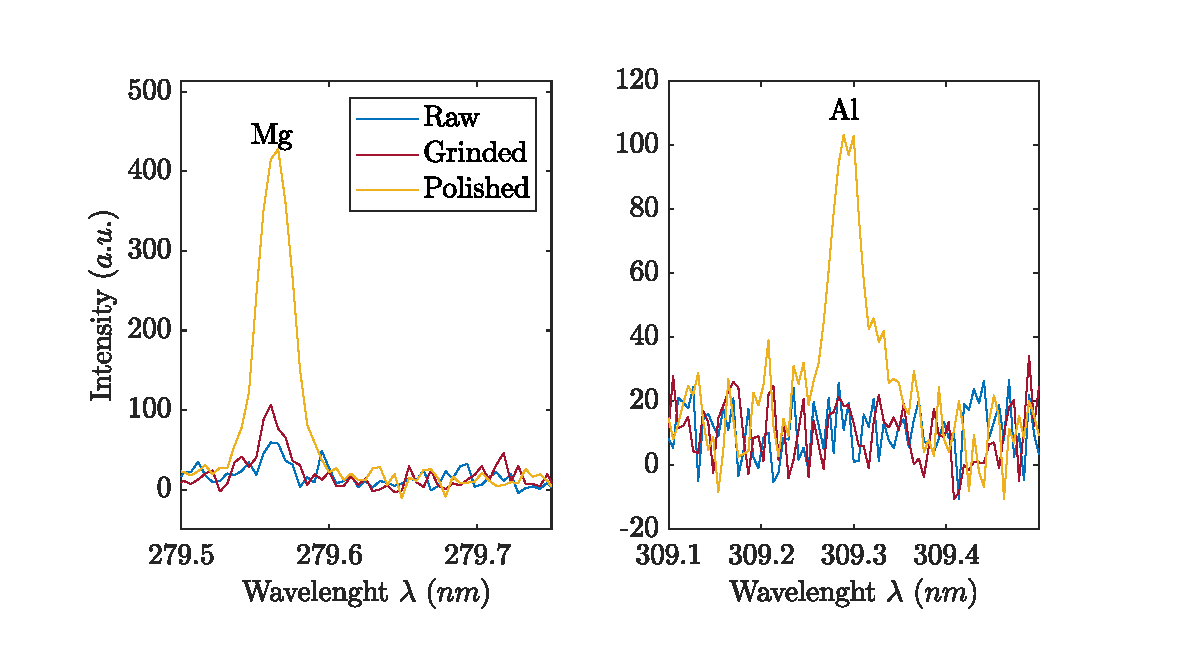
\includegraphics[width = \textwidth]{chapter_5/LIBS/spectra_comparison/dist_15pc_first.pdf} 
    %\caption{Width and depth measurements of LIBS craters performed with a 3D microscope. The peaks are ordered from left to right accordingly to the number of pulses.}
    %\label{fig:3d_microscope_craters}
 \end{figure}

\vspace*{-68pt}
\begin{figure}[H]
    \centering
    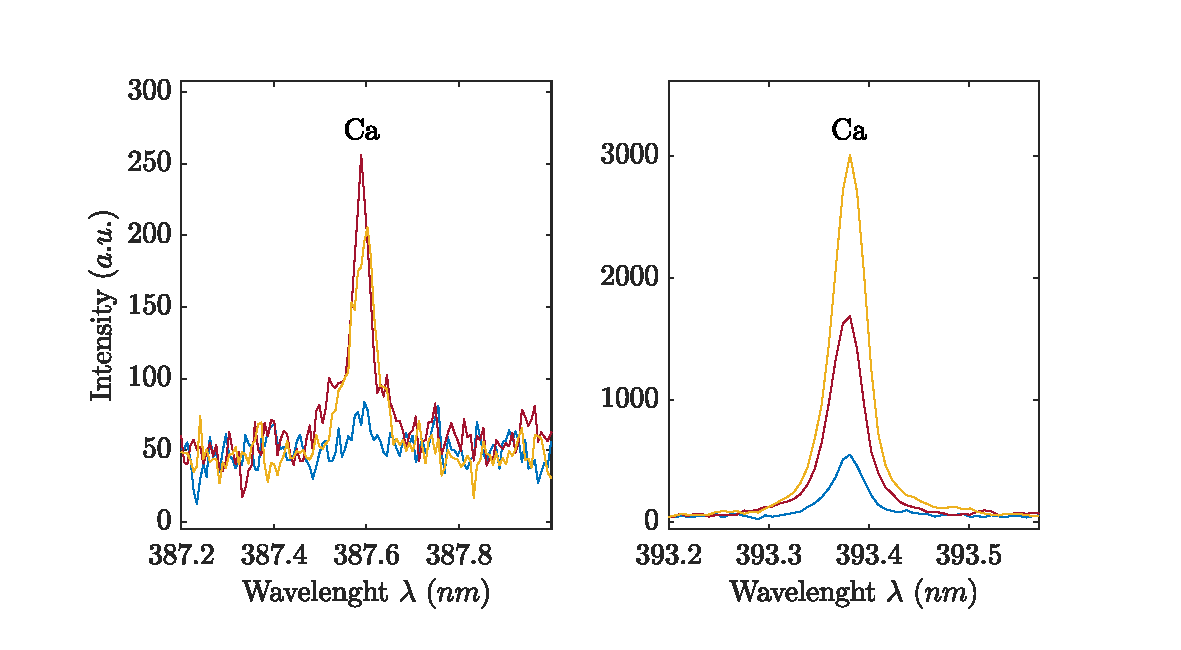
\includegraphics[width = \textwidth]{chapter_5/LIBS/spectra_comparison/dist_15pc_second.pdf} 
    %\caption{Width and depth measurements of LIBS craters performed with a 3D microscope. The peaks are ordered from left to right accordingly to the number of pulses.}
    %\label{fig:3d_microscope_craters}
 \end{figure}

\vspace*{-68pt}
\begin{figure}[H]
    \centering
    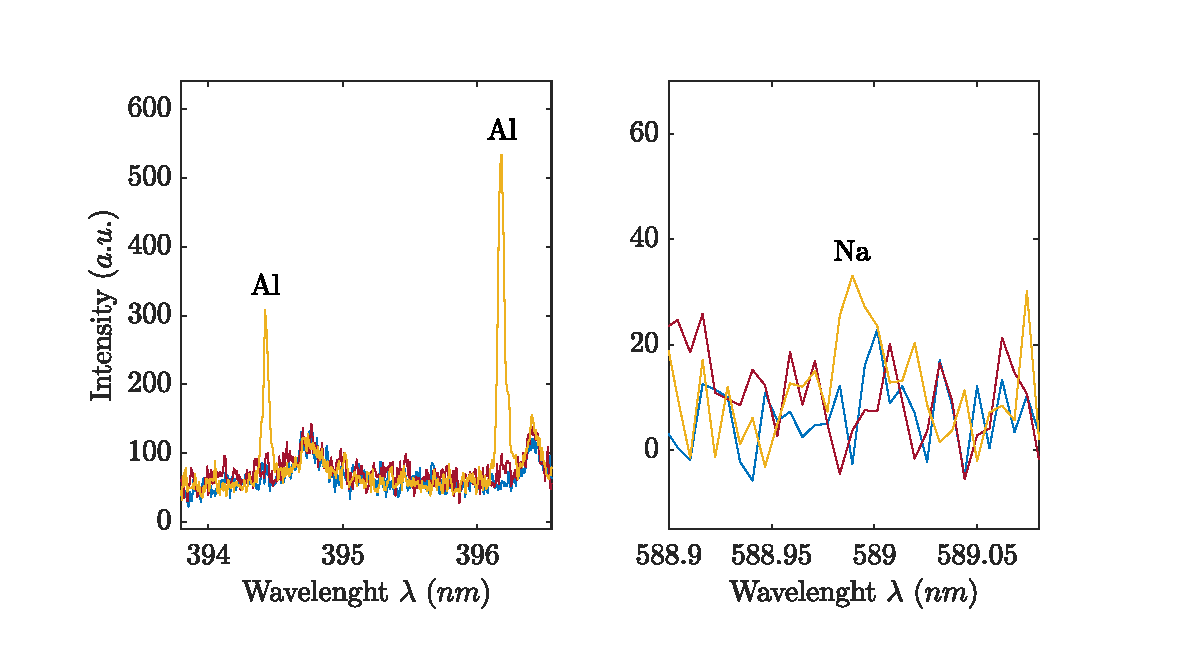
\includegraphics[width = \textwidth]{chapter_5/LIBS/spectra_comparison/dist_15pc_third.pdf} 
    %\caption{Width and depth measurements of LIBS craters performed with a 3D microscope. The peaks are ordered from left to right accordingly to the number of pulses.}
    %\label{fig:3d_microscope_craters}
 \end{figure}

In these last batch of plots it is notable that, even with distilled water, the presence of contaminants like \ce{Ca}, \ce{Mg} and \ce{Na} has still been detected on the sample surface. 

 \begin{figure}[H]
    \centering
    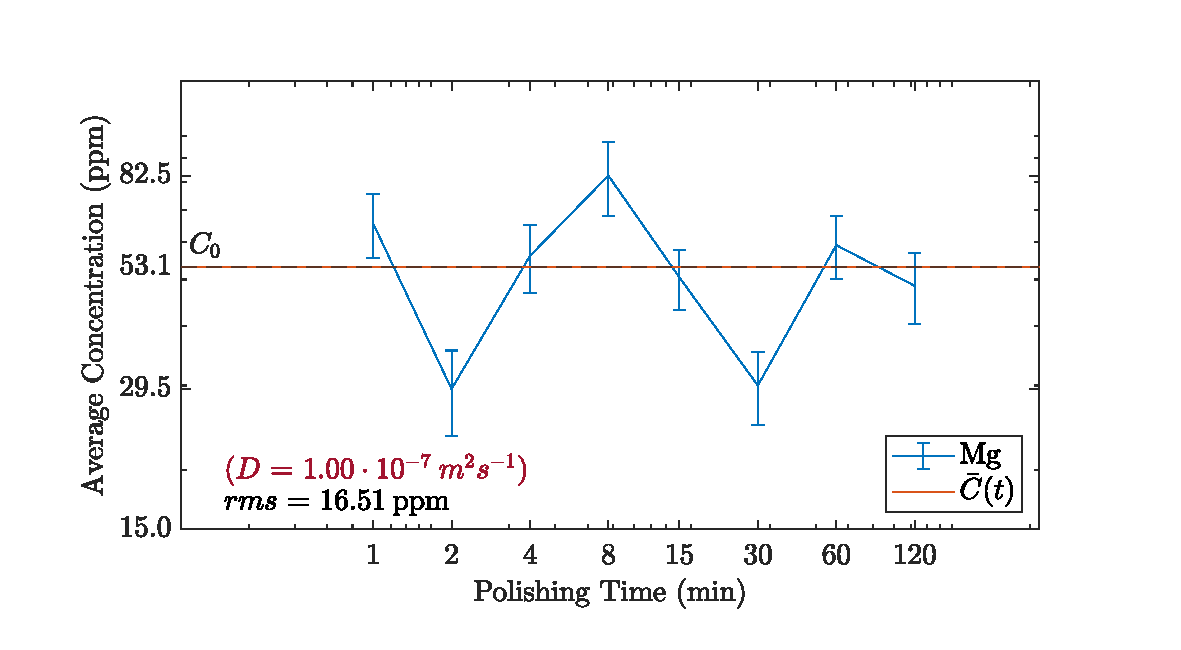
\includegraphics[width = \textwidth]{chapter_5/LIBS/data_fit/fit_dist_15pc_Mg.pdf} 
 \end{figure}

 \begin{figure}[H]
    \centering
    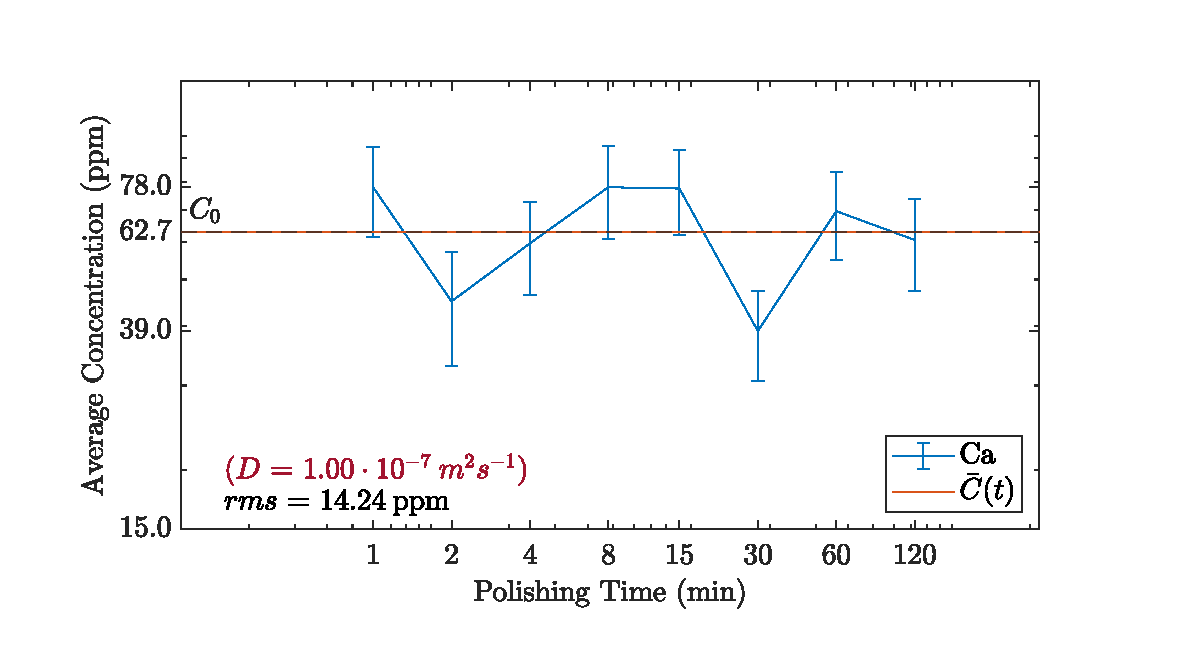
\includegraphics[width = \textwidth]{chapter_5/LIBS/data_fit/fit_dist_15pc_Ca.pdf} 
    %\caption{Width and depth measurements of LIBS craters performed with a 3D microscope. The peaks are ordered from left to right accordingly to the number of pulses.}
    %\label{fig:3d_microscope_craters}
 \end{figure}
    \vspace{-40pt}
 \begin{figure}[H]
    \centering
    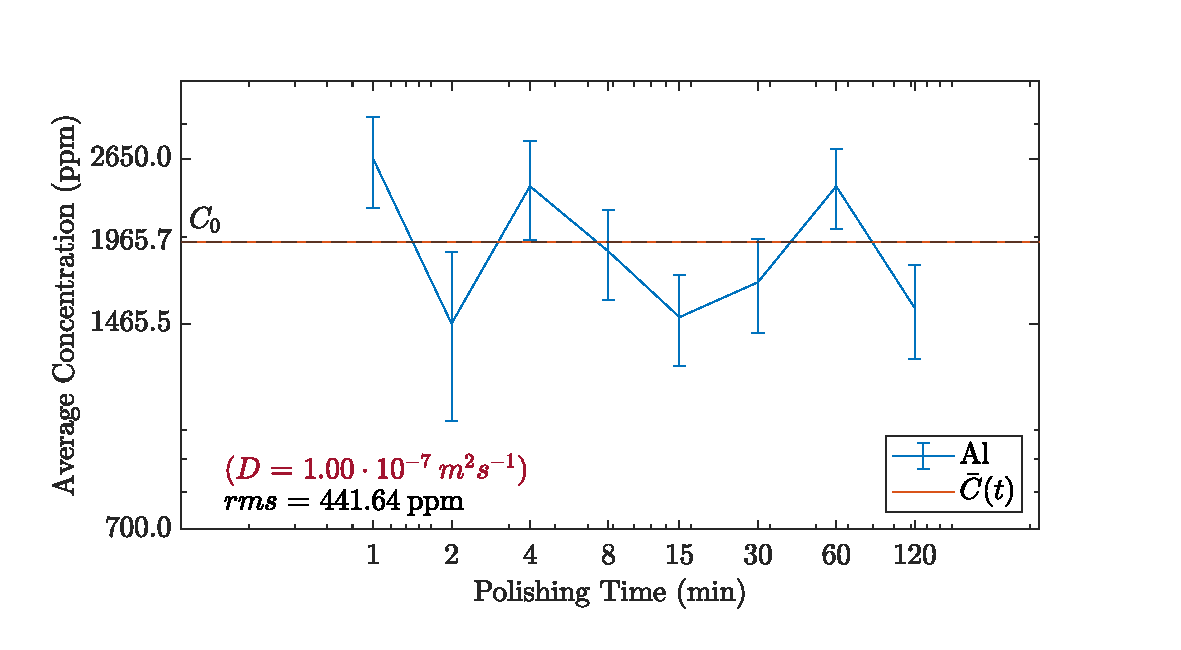
\includegraphics[width = \textwidth]{chapter_5/LIBS/data_fit/fit_dist_15pc_Al.pdf} 
    %\caption{Width and depth measurements of LIBS craters performed with a 3D microscope. The peaks are ordered from left to right accordingly to the number of pulses.}
    %\label{fig:3d_microscope_craters}
 \end{figure}

Even in this case, none of the data related to the contaminants could be fitted to the function we proposed for describing the diffusion process. Notably, all the concentrations evolutions exhibit a less pronounce decreasing behavior, and they all seem to remain roughly constant throughout the polishing process.

\subsubsection{Comparison between Different Types of Water}
\label{subsubsec:comparison_between_waters}

\begin{figure}[H]
   \centering
   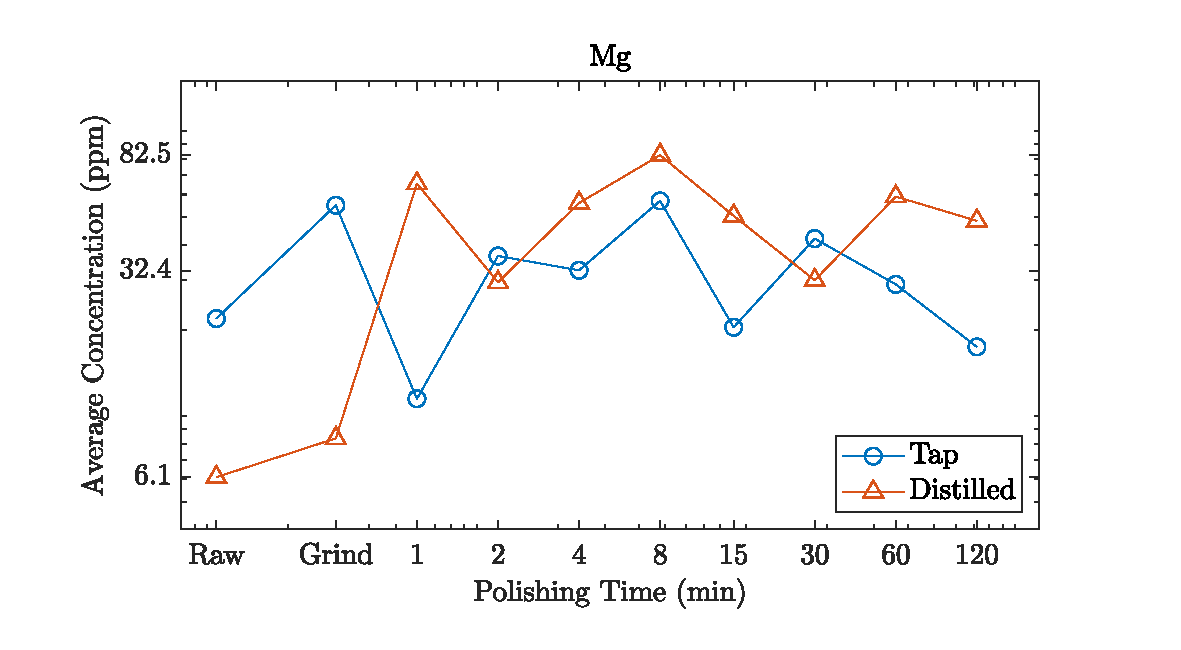
\includegraphics[width = \textwidth]{chapter_5/LIBS/Water_comparisons/Water_comp_Mg.pdf} 
   \vspace*{-30pt}
   \caption{Comparison between the magnesium concentration relative to the two types of water.}
   \label{fig:water_comp_mg}
\end{figure}


\begin{figure}[H]
   \centering
   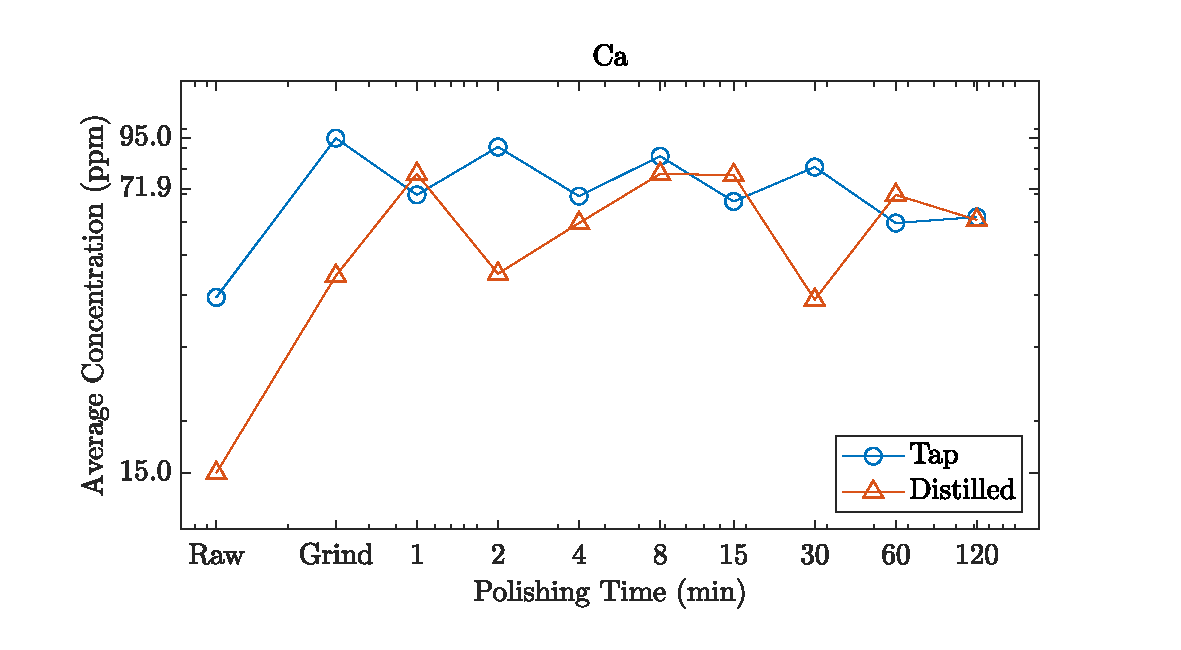
\includegraphics[width = \textwidth]{chapter_5/LIBS/Water_comparisons/Water_comp_Ca.pdf} 
   \vspace*{-30pt}
   \caption{Comparison between the calcium concentration relative to the two types of water.}
   \label{fig:water_comp_ca}
\end{figure}


\begin{figure}[H]
   \centering
   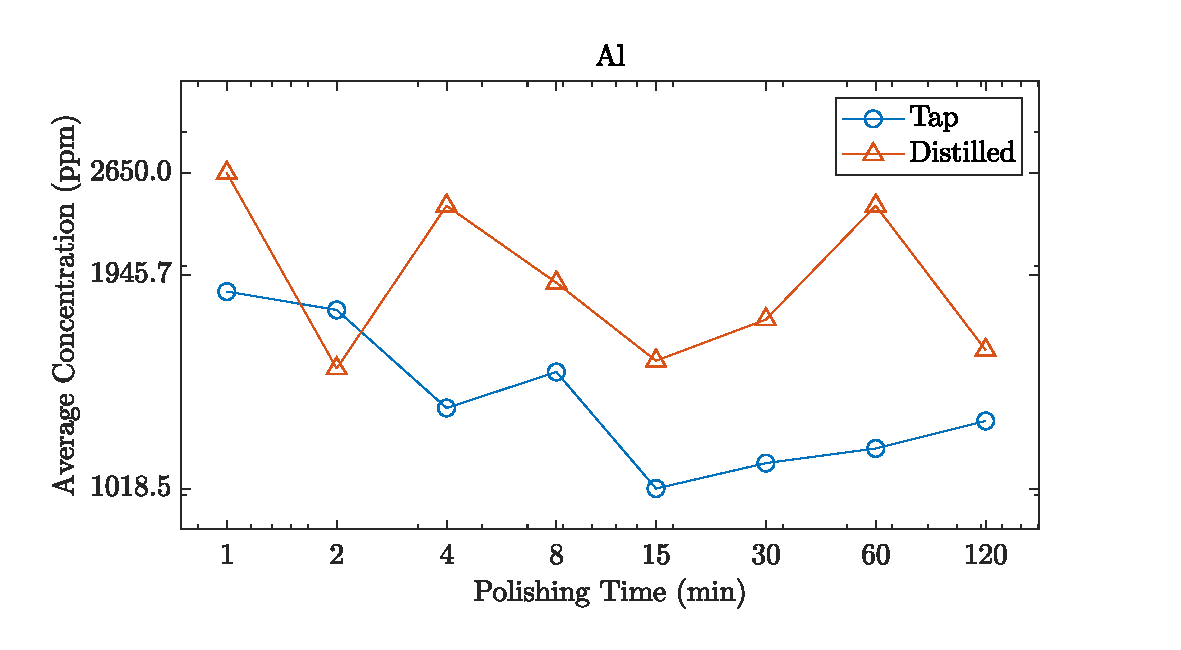
\includegraphics[width = \textwidth]{chapter_5/LIBS/Water_comparisons/Water_comp_Al.pdf} 
   \vspace*{-30pt}
   \caption{Comparison between the aluminum concentration relative to the two types of water.}
   \label{fig:water_comp_al}
\end{figure}

From these graphs it is clear that, not only there is still presence of alkali metal contaminants even for distilled water, but the detected concentration is equal, or even slightly higher, to the case of tap water. In addition, Figure~\ref{fig:water_comp_al} shows an average concentration of aluminum that is almost a factor of two higher at every polishing time for the case of distilled water.

\section{Considerations}
\label{sec:considerations}
The most important consideration that can be drawn from all the LIBS data is the fact that diffusion cannot be the main driving mechanism under the presence of contaminants at the surface of the glass. The trend for the contaminants' concentration was decreasing for all the samples measured, and Fick's laws (Equation~\ref{eq:second_fick}) cannot describe in any way a decreasing concentration of particles when there is a constant source of diffusant, like in the case of polishing. Additionally, such a high presence of contaminants even after just one minute of polishing, would've required a diffusion constant way above the values that are reasonably associated with a diffusion process into a solid sample.
\\
A possible hypothesis is that the major cause of the contamination could be caused by the presence of "microcracks" (shown in Figure~\ref{fig:micro_cracks}) that are partially already on the surface of the raw sample, and are increased by the mechanical effect of the grinding. The silica gel layer, infused with the elements present in the polishing suspension, can flow into the cracks thanks to the local high temperatures caused by friction during polishing.
\\
High polishing times partially interfere with the process by removing some of the defects that were generated during the previous stage, and, consequently, decreasing the detected concentration of contaminants.
\\
It is not fully clear why the concentration of the polish does not seem to have a definite influence on the process (Figure~\ref{fig:tap_conc_comp_al}). A higher density of polishing agent should impact both the concentration of external elements inside the silanol layer, and should also increase the MRR (material removal rate), therefore affecting the speed of which the cracks are being polished from the surface.
\\
It is notable that in XPS data (Chapter~\ref{sec:xps_results}), the concentration of aluminum seems to instead increase as the polished concentration increased. This could suggest that the polish concentration is more relevant for the processes that happen at the outermost layers of the surface, that are the ones measured by XPS.
\\
Another clear result is that using distilled water does not prevent at all the introduction of mineral impurities into the sample. The presence of these species in the tools used for the processes (measured in Chapter~\ref{subsec:measurements_pol_components}) is apparently enough to contaminate the glass with the same magnitude as using tap water as solvent. As a matter of fact, distilled water seems to indirectly favor the contamination from the polishing agent, as shown in Figure~\ref{fig:water_comp_al}, probably caused by the increase in pH level for the solution formed in distilled water (Table~\ref{table:solution_ph}).

\chapter{Conclusions and Future Developments}
\label{ch:conclusions_and_dev}
For what regards the use of LIBS for analyzing glass surfaces, its versatility and speed makes this experimental technique an appropriate choice for this type of measurements. An analogous investigation carried out with a different spectroscopy, for example XPS, would have taken way longer times and would have required many more samples. The possibility of interrupting the processing of the glass, instantly taking the measurements, and resuming the polishing of the sample right away, cannot be granted by any other analysis method. As an example, the XPS measurement we presented in this thesis required a different sample for every polishing parameter that we were investigating, and the results took few weeks to be obtained.
\\
The main issue of LIBS stands in its high variability, small differences in the characteristics of the laser induced plasma can have non-uniform impact on the emission, that are not directly correlated with differences in concentrations of the elements in the sample. This problem was even more evident in our case due to the fact that only one pulse per measurement was performed, and by the fact that the laser wavelength in the CORALIS apparatus was not ideal to investigate glass samples. The inconsistencies were partially mitigated by the use of the analysis procedure presented in Chapter~\ref{subsec:analysis_workflow}, that allowed to estimate the plasma parameters and to simulate the emission accordingly. However, any further investigation should still be carried out with a more appropriate laser wavelength.
\\
\\
Regarding the glass processing phase, more automatized polishing and grinding methods should be employed to reduce variability caused by human handling. Specifically, one of the main issues stood in the method used to deliver the polishing suspension on the polishing cloth. We provided the slurry on the cloth whenever the latter started to present signs of dryness, the frequency of the delivery varied a lot from session to session. Even though it probably did not influence the results, it was a variable that should be more controlled in future similar analyses.
\\
The results related to the use of distilled water shown that the water itself is not the only source of mineral contaminants. From a point of view of future researches, specifically cleaned instruments and polishing agents with high purity must be utilized in order to ensure the absence of any contamination source. Under a practical point of view, we showed that even by using distilled water for the polishing suspension and to clean the instrumentation, and by employing factory-new polishing cloths and grinding paper, contamination could not be avoided at all. Tap water is therefore the most reasonable choice.
\\
\\
Lastly, any further investigation on this topic should focus on developing a theoretical model that could make quantitative predictions in accordance to the measured data.